 \documentclass[a4paper,fleqn,usenatbib]{mnras}

%font
\usepackage{newtxtext,newtxmath}
% Depending on your LaTeX fonts installation, you might get better results with one of these:
%\usepackage{mathptmx}
%\usepackage{txfonts}

% Use vector fonts, so it zooms properly in on-screen viewing software
% Don't change these lines unless you know what you are doing
\usepackage[T1]{fontenc}
\usepackage{ae,aecompl}

% Only include extra packages if you really need them. Common packages are:
\usepackage{graphicx}	% Including figure files
\usepackage{amsmath}	% Advanced maths commands
\usepackage{amssymb}	% Extra maths symbols

%\usepackage{caption} %doesn't work!!!!!
\usepackage{threeparttable}


\graphicspath{{figures/}}

%%%%%%%%%%%%%%%%%%%%%%%%%%%%%%%%%%%%%%%%%%%%%%%%%%

%%%%% AUTHORS - PLACE YOUR OWN COMMANDS HERE %%%%%

% Please keep new commands to a minimum, and use \newcommand not \def to avoid
% overwriting existing commands. Example:
%\newcommand{\pcm}{\,cm$^{-2}$}	% per cm-squared

%%%%%%%%%%%%%%%%%%%%%%%%%%%%%%%%%%%%%%%%%%%%%%%%%%

%%%%%%%%%%%%%%%%%%% TITLE PAGE %%%%%%%%%%%%%%%%%%%

% Title of the paper, and the short title which is used in the headers.
% Keep the title short and informative.
\title[SZ effect in SHELA cluster candidates]{Draft: The Atacama Cosmology Telescope: SZ-based masses of IR-selected cluster candidates from the SHELA survey}

% The list of authors, and the short list which is used in the headers.
% If you need two or more lines of authors, add an extra line using \newauthor
\author[B. Fuzia et al.]{
Brittany Fuzia,$^{1}$\thanks{E-mail: bjf13d@my.fsu.edu}
Lalitwadee Kawinwanichakij,$^{2}$
Eli Rykoff,$^{3}$
Nicola Mehrtens,$^{2}$
\newauthor ACT and SHELA collaborators, 
including
Kevin Huffenberger,$^1$ 
Casey Papovich$^{2}$, 
\newauthor Bruce Partridge, Crist\'obal Sif\'on
\\
% List of institutions
$^{1}$Dept of Physics, Florida State University, Tallahassee, FL 32301, USA\\
$^{2}$Dept of Physics and Astronomy, Texas A\&M University, College Station, TX 77843, USA\\
$^{3}$ SLAC National Accelerator Laboratory, Menlo Park, CA 94025, USA\\
}

% These dates will be filled out by the publisher
\date{Accepted XXX. Received YYY; in original form ZZZ}

% Enter the current year, for the copyright statements etc.
\pubyear{2018}

% Don't change these lines
\begin{document}
\label{firstpage}
\pagerange{\pageref{firstpage}--\pageref{lastpage}}
\maketitle

% Abstract of the paper
\begin{abstract}
We analyze the stacked Sunyaev-Zel\text{'}dovich (SZ) temperature decrement for an infrared-selected sample of galaxy cluster candidates from the Spitzer-HETDEX Exploratory Large Area (SHELA) Survey. The clusters are found in combined optical and infrared SHELA data using the redMaPPer algorithm. We separate the sample into two richness bins: $10 \leq \lambda < 20$, and $\lambda \geq 20$. The average redshifts for the samples are 0.71 and 0.80. IR selection allows us to probe clusters at higher redshifts than typical with optically-selected samples, with objects less massive than those typical with SZ surveys. In the stacking analysis, Atacama Cosmology Telescope (ACT) measurements show a temperature decrement at 148 GHz.  Excess emission at the 220 GHz SZ null we attribute to dust emission from the cluster member galaxies. We correct for dust emission in the 148 GHz stack using the 220 GHz profile as the dust template. We extrapolate the 220 GHz signal to 148 GHz to based on a dust spectral energy distribution (SED) fit to data from the Herschel Stripe 82 (HerS) survey.  We use a Markov Chain Monte Carlo to clean our decrement using the extrapolated 220 GHz dust profile and simultaneously fit for the cluster mass, using a universal galaxy cluster pressure profile for the average SZ signal.  We find a mean mass of $M_{500} = (1.7 \pm 0.8)\times 10^{13} M_{\odot}$ and $(4.9 \pm 1.7) \times 10^{13}$ $M_{\odot}$, respectively, for the poorer and richer samples. These masses are 1.9 and 2.2 times larger than what we find when neglecting the dust correction, indicating substantial fill-in of the SZ decrement from the cluster dust emission, up to 80 percent in terms of $Y_{500}$, although with large uncertainty. We compare our SZ masses to two redMaPPer-based cluster scaling relations for richness and find that the SZ mass is lower than predicted by the richness, even after correcting for dust emission.  Part of the discrepancy may be due to a differing interpretation of richness for selection in the infrared.
%We find a high stellar-to-total mass fraction in all richness bins. 
\end{abstract}

% Select between one and six entries from the list of approved keywords.
% Don't make up new ones.
\begin{keywords}

\end{keywords}

%%%%%%%%%%%%%%%%%%%%%%%%%%%%%%%%%%%%%%%%%%%%%%%%%%

%%%%%%%%%%%%%%%%% BODY OF PAPER %%%%%%%%%%%%%%%%%%


%%%%%%%%%%%%%%%%%%%%%%%%%%%%%%%
%INTRODUCTION
%%%%%%%%%%%%%%%%%%%%%%%%%%%%%%%
\section{Introduction}
Clusters of galaxies are the largest gravitationally bound structures in the universe. They make powerful cosmological probes because they sample the maxima of the primordial density field.  Various cluster observables relate to each other with scaling laws and these laws make clusters useful tools to gain insight into large-scale structure, galaxy evolution, dark matter dynamics, and cosmological parameters \citep{2005RvMP...77..207V,2013SSRv..177..247G}. The thermal Sunyaev-Zel'dovich (SZ) spectral distortion of the Cosmic Microwave Background (CMB) allows for indirect measurements of one of the most important observables---total galaxy cluster mass---and can identify clusters to high redshift \citep{1972CoASP...4..173S, 2002ARA&A..40..643C}. 
The SZ effect occurs when CMB photons scatter from the hot electron gas in the intracluster medium. Fewer than $\sim$1 percent of photons interact and gain energy through inverse Compton scattering, altering the observed CMB spectrum and resulting in a characteristic spectral dependence for the SZ effect: a flux decrement for frequencies below 217 GHz and a flux increment for higher frequencies \citep{1999PhR...310...97B,2002ARA&A..40..643C}.
The magnitude of the effect is proportional to the Comptonization parameter (the integrated electron pressure), and the pressure is proportional to the depth of the gravitational potential well.  Therefore the amplitude of the SZ signal depends on the mass of the cluster.
Using the SZ effect for cosmology requires an understanding of this relationship between halo mass and the SZ observable, which is often expressed as the Comptonization parameter integrated over the cluster's solid angle. 
Since the SZ effect is a distortion of the CMB's spectrum, the signal does not decrease with distance the way that the cluster brightness does, and so the SZ effect is an efficient way to find high-redshift clusters, limited only by the mass of the cluster and the sensitivity of the telescope.

At high mass, $M \gtrsim 10^{15}$ $M_\odot$, current SZ searches can already find halos efficiently at all redshifts, but at lower mass, $M \lesssim 10^{14}$ M$_{\odot}$, it becomes more difficult. These lower mass halos are interesting because their smaller potential wells have a harder time holding onto their gas, and they are laboratories for star formation and AGN feedback \citep{2015MNRAS.448.2085L,2013A&A...555A..66L}.  Although studies of low mass halos using the SZ effect will become more common as CMB telescopes become more sensitive, for now we depend on stacking, or averaging, multiple clusters that have been detected by other means.  Stacking lets us use the SZ effect down to these lower masses, as it averages out contributions from the CMB and detector noise \citep{2013ApJ...767...38S, 2011A&A...536A..12P, 2011ApJ...736...39H}.

At low redshift, optical surveys can identify clusters efficiently with multiband overdensity finders: e.g. MaxBCG \citep{2007ApJ...660..221K}, redMaPPer \citep{2014ApJ...785..104R}, and CAMIRA \citep{2014MNRAS.444..147O}.
At higher redshift, the infrared becomes an efficient avenue: e.g. MaDCoWS \citep{2014ApJS..213...25S}, ISCS 
\citep{2008ApJ...684..905E}, IDCS \citep{2012ApJ...753..164S}.

The SZ signal of low-richness, optically-selected clusters is less than expected from SZ mass--richness and weak lensing mass--richness relationships, which are usually calibrated with high-richness clusters.  \citep{2011A&A...536A..12P,2012PhRvD..85b3005D,2013ApJ...767...38S,2016arXiv160508770S}. Several possible explanations for this discrepancy are radio or infrared point source contamination of the SZ signal, line-of-sight projections contaminating richness measurements, cluster miscentering, or a lower amplitude for the mass-richness relation. Solving this discrepancy is vital so that scaling relations for clusters, and therefore cluster physics, are understood over a wide mass range, allowing clusters to be used to their full cosmological potential.

In this work, we stack measurements of the SZ signal in data from the Atacama Cosmology Telescope (ACT) on cluster candidates selected from multifrequency imaging, including Spitzer data from the SHELA survey, by the redMaPPer algorithm.  This sample is higher in redshift and lower in mass than many other samples. Using Herschel and Planck data, we correct the stacked SZ decrement for contamination from dusty sources, and fit for a halo mass based on the cleaned SZ signal. We also compare the sample's average stellar mass and mass-richness relationship.
We adopt the flat $\Lambda$CDM cosmology from the Planck 2013 data release \citep{2014A&A...571A..16P} with $H_{0}$ = 67.9 km s$^{-1}$ Mpc$^{-1}$, $\Omega_{\rm m}$ = 0.307, $\Omega_{\rm \Lambda}$ = 0.693. The SZ signal and mass $M_{500}$ is measured out to $R_{500}$, which is the radius enclosing 500 times the critical density at a given redshift.

This paper is organized as follows: In Section \ref{sec:data} we introduce the cluster sample, the ACT and ACTPol data, and the Herschel data used in this analysis. In Section \ref{sec:methods} we describe the methods we used to analyze the data. These include the filtering and stacking procedures, calculation of the covariance matrices, and a discussion of the noise and signals that contribute to the stacked profiles. We describe our resulting multifrequency stacked profiles 
%in Section \ref{sec:multifreqprof}, 
and discuss our methods for removing dust contamination. We describe our fitting procedure, including the SZ and pressure profile we use to translate our SZ signal into a cluster mass. In section \ref{sec:results}, we present the results of our analysis and discuss how our SZ mass scales with stellar mass and richness. Section \ref{sec:conclusions} concludes with a summary of the analysis and results.


%%%%%%%%%%%%%%%%%%%%%%%%%%%%%%% 
%DATA 
%%%%%%%%%%%%%%%%%%%%%%%%%%%%%%% 
\section{Data} \label{sec:data}

\subsection{Cluster Sample}
The sample contains IR and optically selected redMaPPer cluster candidates from the Spitzer-HETDEX Exploratory Large Area survey  \citep{2016ApJS..224...28P}. SHELA is a 24 deg$^2$ IRAC survey in a low IR background region of Stripe 82, centered at a right ascension of 1$^{\rm h}$22$^{\rm m}$00$^{\rm s}$ on the celestial equator, and extending $\pm$6.5$^{\circ}$ in right ascension and $\pm$1.25$^{\circ}$ in declination. The SHELA survey region also includes DES $ugriz$ imaging. Multiwavelength coverage in the same field includes SDSS, HETDEX, and DECam in the optical, NEWFIRM in K-band, Herschel in the sub-mm, and ACT in the microwave. 

The IR and optical imaging are passed through the redMaPPer algorithm \citep{2014ApJ...785..104R}, resulting in a catalog of 8674 groups and clusters, of which 701 have a richness $\lambda \geq 10.$ Richness is a measure of how many galaxies belong to a cluster. In redMaPPer, it is defined as the sum of the membership probabilities for the galaxies within a cluster. We use clusters with richnesses $\lambda \geq 10$, and break these into two richness bins: $10 \leq \lambda < 20$ and $\lambda \geq 20$. Two are rich clusters already detected in the ACT SZ cluster sample \citep{2013JCAP...07..008H}. We discard any SHELA clusters within 3 arcminutes of the ACT detected clusters before conducting a stacking analysis, leaving 623 and 75 clusters in the lowest and highest richness bin, respectively. None of the remaining objects are detected individually in SZ by ACT, so their individual masses must be roughly $\leq 10^{14}$ M$_\odot$, ACT's approximate mass limit.


\subsection{ACT Microwave Data}
We use ACT data to measure the SZ decrement and null signals. ACT is a six-meter millimeter wave telescope that resides at an altitude of 5200 meters on Cerro Toco in the Atacama Desert of Chile. It surveys the CMB with high resolution and sensitivity. The first generation of ACT observed during 2007-2010, and had three detector arrays at frequencies of 148, 220, and 277 GHz. These bands were chosen to study the SZ and capture the SZ decrement, null, and increment. ACT surveyed two regions on the sky, the ``southern'' and ``equatorial'' surveys. The southern survey covered 455 deg$^2$ and is centered on declination -53.5$^{\circ}$ \citep{2011ApJ...731..100M}. The equatorial region overlaps with 270 deg$^2$ of Stripe 82 and the entire SHELA survey, covering 504 deg$^2$ and spanning from 20$^{\rm h}$16$^{\rm m}$00$^{\rm s}$ to 3$^{\rm h}$52$^{\rm m}$24$^{\rm s}$ in right ascension and -2$^{\circ}$07$^{\prime}$ to 2$^{\circ}$18$^{\prime}$ in declination \citep{2013JCAP...07..008H}. The second generation of the experiment, ACTPol, was deployed in 2013 and has receivers at 90 and 148 GHz, with triple the sensitivity of ACT and is polarization sensitive. ACTPol has made observations in four deep field patches and one wider field and continues to take data \citep{2014JCAP...10..007N}. The wider ``Deep 5/6'' region overlaps with SHELA, covering 548 deg$^2$ and is centered on the celestial equator, expanding the area covered by ACT.
In this work, we measure the SZ decrement using coadded, source subtracted, ACT temperature maps at 148 GHz from all observing seasons which overlap with the SHELA survey region: seasons 3--4 (2009 and 2010) of ACT and season 2 (2014) of ACTPol. The ACT maps have 0.495 arcmin pixels, while the ACTPol maps have 0.5 arcmin pixels. We use ACT maps that have been repixelized into the ACTPol pixelization to make coadded maps of all available data. %\citep{2011ApJS..194...41S}??. 
We use 220 GHz data from seasons 3--4 of ACT, which is approximately the SZ null, to constrain contamination from thermal dust emission. These maps are also repixelized into the ACTPol pixelization. The beam sizes are 1.4 arcmin at 148 GHz, and 1.0 arcmin at 220 GHz.

\subsection{Herschel Submillimeter Data}
To measure dust emission from cluster member galaxies, we use far-IR data from the Herschel Stripe 82 (HerS) survey, which consists of maps at 250, 350, and 500 $\mu$m (or 1200, 857, 600 GHz) observed with \textit{Herschel}/SPIRE \citep{2014ApJS..210...22V}. The survey covers 79 deg$^2$, spanning 13$^{\circ}$ to 37$^{\circ}$ in right ascension and -2$^{\circ}$ to +2$^{\circ}$ in declination. 
The SPIRE beams are 18.2, 25.2, and 36.3 arcsec at 1200, 857, 600 GHz, respectively. In addition to the maps, in this work we use the band-merged source catalog from the HerS team, which contains compact source flux densities and uncertainties in each band. The HerS team assumed sources are point-like and they identified them using the IDL software package STARFINDER \citep{2000A&AS..147..335D}. They produced the band-merged catalog using the De-blended SPIRE Photometry (DESPHOT) algorithm, which uses sources from the 1200 GHz band as a prior for the other frequencies \citep{2010MNRAS.409...48R}.


%%%%%%%%%%%%%%%%%%%%%%%%%%%%%%%
%METHODS
%%%%%%%%%%%%%%%%%%%%%%%%%%%%%%%
\section{Methods} \label{sec:methods}

\subsection{SZ Profiles}
The SZ signal can be expressed as a change in CMB temperature by: 
\begin{equation}
\centering
  \frac{\Delta T}{T_{CMB}} = y( \theta ) \, f( x )
\end{equation}
where $x = \frac{h \nu}{k T}$ and $f(x) = x ({e^{x} + 1})/{(e^{x}-1)} - 4$ contains the frequency dependence of the SZ effect. The Compton parameter $y$ is proportional to pressure integrated along the line of sight \citep{1972CoASP...4..173S,1970CoASP...2...66S}:
\begin{equation}
  y = \frac{\sigma_{T}}{m_{e} c^{2}} \int dl\  P(\theta, l) \end{equation}
To translate our stacked temperature profile into a mass measurement, we use a universal pressure profile (UPP) of \cite{2010A&A...517A..92A} [A10], which is calibrated using low-redshift X-ray clusters from REXCESS \citep{2007A&A...469..363B}. \citeauthor{2010A&A...517A..92A} fit a generalized Navarro-Frenk-White profile which allows for a normalization that varies with mass and redshift and a mass-dependent deviation from self-similarity in the shape of the profile. In this model, the pressure at any radius $r$ (or $x' \equiv r/R_{500}$) is:

\begin{equation}
P(r) = P_{500} \bigg[ \frac{M_{\rm SZ,500}}{3x10^{14} h^{-1}_{70} M_{\odot}} \bigg]^{\alpha_{p} + \alpha^{\prime}_{p}(x')} \textbf{p}(x') \ h^{2}_{70} \ keV \ cm^{-3}
\end{equation}
where $P_{500}$ is the normalization of the pressure profile at a radius of 500 times the critical density at a given redshift:
\begin{equation}
P_{500} = 1.65 \times 10^{-3} E(z)^{8/3} \bigg[\frac{M_{500}}{3 \times 10^{14} h_{70}^{-1} M_{\odot}}\bigg]^{2/3} h_{70}^2 keV cm^{-3}
\end{equation}
\textbf{p}$(x')$ is the dimensionless universal pressure profile:
\begin{equation}
\textbf{p}(x') = \frac{P_{0}}{(c_{500} x')^{\gamma} [1 + (c_{500} x')^{\alpha}]^{(\beta-\gamma)/\alpha}}
\end{equation}
and $\alpha^{\prime}_{p}(x')$ describes the deviation from self-similiarity:
\begin{equation}
\alpha^{\prime}_{p}(x') = 0.10 - (\alpha_{p} + 0.10) \frac{(x'/0.5)^{3}}{1. + (x'/0.5)^{3}}
\end{equation}
with $\alpha_p$ = 0.12.
Using local clusters with XMM-Newton data, \cite{2013A&A...550A.131P} update the best-fit parameters for the UPP to [$P_{0},c_{500},\gamma,\alpha,\beta$] = [6.51,1.81,0.31,1.33,4.13], which we adopt in this paper.


\subsection{Map Filtering and Stacking}
Before stacking, we filter the maps using a conservative high-pass filter designed to remove large scale CMB fluctuations without altering the small scale cluster signal. To avoid bias, we design a filter independent of any assumed cluster shape.
Our filter is a Fourier-space high-pass filter that we define in terms of its low-pass complement.  The low-pass complement in real space is an apodized top-hat: unity inside $3'$ radius and tapering to zero outside of $5'$ with a cosine transition. Thus our high-pass filter removes the large scale features in the map, and barely touches small harmonic scales. Our filter is not matched to any specific cluster profile, and preserves the small-scale detector white noise.  When compared, all maps, simulations, and model cluster profiles are subjected to this same filter.  We tested that our results are robust when introducing beam smoothing into our filter. The filter is the same high-pass filter used for the analysis, but convolved with the beam at 148 GHz to reduce pixel-scale white noise. This resulted in smoother, shallower profiles and mass measurements similar to those reported in this analysis, but with higher uncertainty as there was more bin to bin covariance.

%\subsection{Stacking Procedure}
The cluster candidates were not individually detected in SZ by ACT. To increase the signal-to-noise we stack, or average, observations of the clusters together into 30 annular bins, centered on the reported cluster positions, out to a radial separation of nine arcminutes. CMB and white noise fluctuations have zero mean, therefore stacking observations partially averages out these noise fluctuations. The center of each pixel determines where the measurement is binned.

We can write our stacked profiles as a sum of the beam-convolved signals ($b \ast P)(\theta)$ and noise ($n$):
\begin{eqnarray}
  \label{eq:prof148}
  P^{148} &=& b^{148} \ast ( P^{\rm SZ} + \alpha_{\rm true} P^{\rm dust,220} + n^{\rm CMB} ) + n^{\rm det,148}  \\
%\end{equation}
%\begin{equation}
  \label{eq:prof220}
  P^{220} &=& b^{220} \ast ( P^{\rm dust,220} + n^{\rm CMB} ) + n^{\rm det,220}
\end{eqnarray}

The dust SED provides $\alpha_{\rm true}$, the amount of the 220 GHz dust signal that is present in the 148 GHz data.
There is little SZ signal at 220 GHz, so we can use this profile to clean the 148 GHz stack by extrapolating the dust emission shape between bands by estimating $\alpha$, which we measure by fitting a dust SED to the total flux density from sources in the HerS survey catalog. When we subtract the 220 GHz channel we deconvolve the beam at 220 GHz and reconvolve with the beam at 148 GHz.

\subsection{Covariance Matrices}

\begin{figure}
\centering
  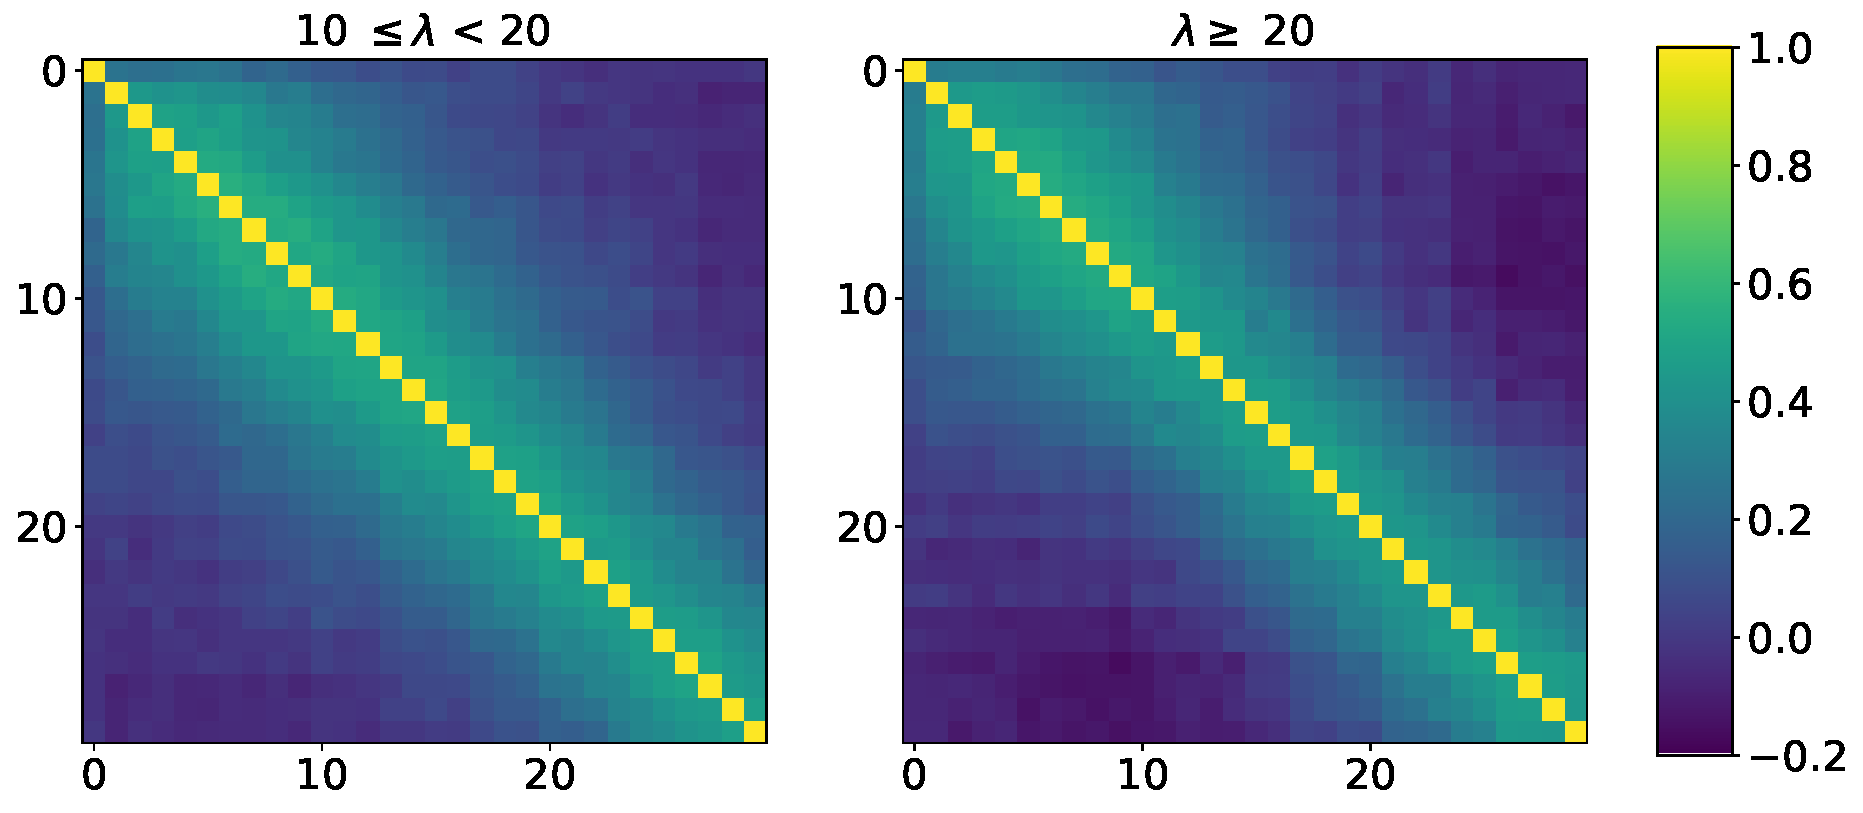
\includegraphics[width=\columnwidth]{correlation_1600_coadd_act_actpol_148_tophat_both.pdf}
  \caption{Correlation matrices for the stacked pressure profiles at 148 GHz for the two richness bins, $10 \geq \lambda < 20$ (left) and $\lambda \geq 20$ (right). They are obtained by stacking on 1600 ACT simulations which contain correlations introduced by CMB fluctuations, detector and atmospheric noise for the different observing seasons of ACT used in this analysis.}
  \label{fig:covariance}
\end{figure}

In the ACT frequencies, 148 and 220 GHz, the error in each annular bin of the stacked profile reflects the covariance introduced by CMB fluctuations, detector noise, and atmosphere. The covariance matrix is calculated by carrying out the same filtering and stacking procedure on 1600 simulations that model coadded ACT and ACTPol maps. To do this, we repixelize the ACT maps into the new ACTPol pixelization, and make coadded maps of all of the different seasons and arrays. We use the power spectra of the coadded maps to generate simulations which are then filtered. The covariance is largest in the small angle bins where there are few measurements to average down the noise. The correlation matrix for each richness bin at 148 GHz is shown in Figure \ref{fig:covariance}.  

Errors on the dust SED also figure into our final uncertainties.  
The HerS catalog includes 1$\sigma$ uncertainties for the flux density of each source, which we use by averaging in quadrature for the SED fitting process. 

\subsection{Multifrequency Profiles} \label{sec:multifreqprof}

\begin{figure*}
  \centering
  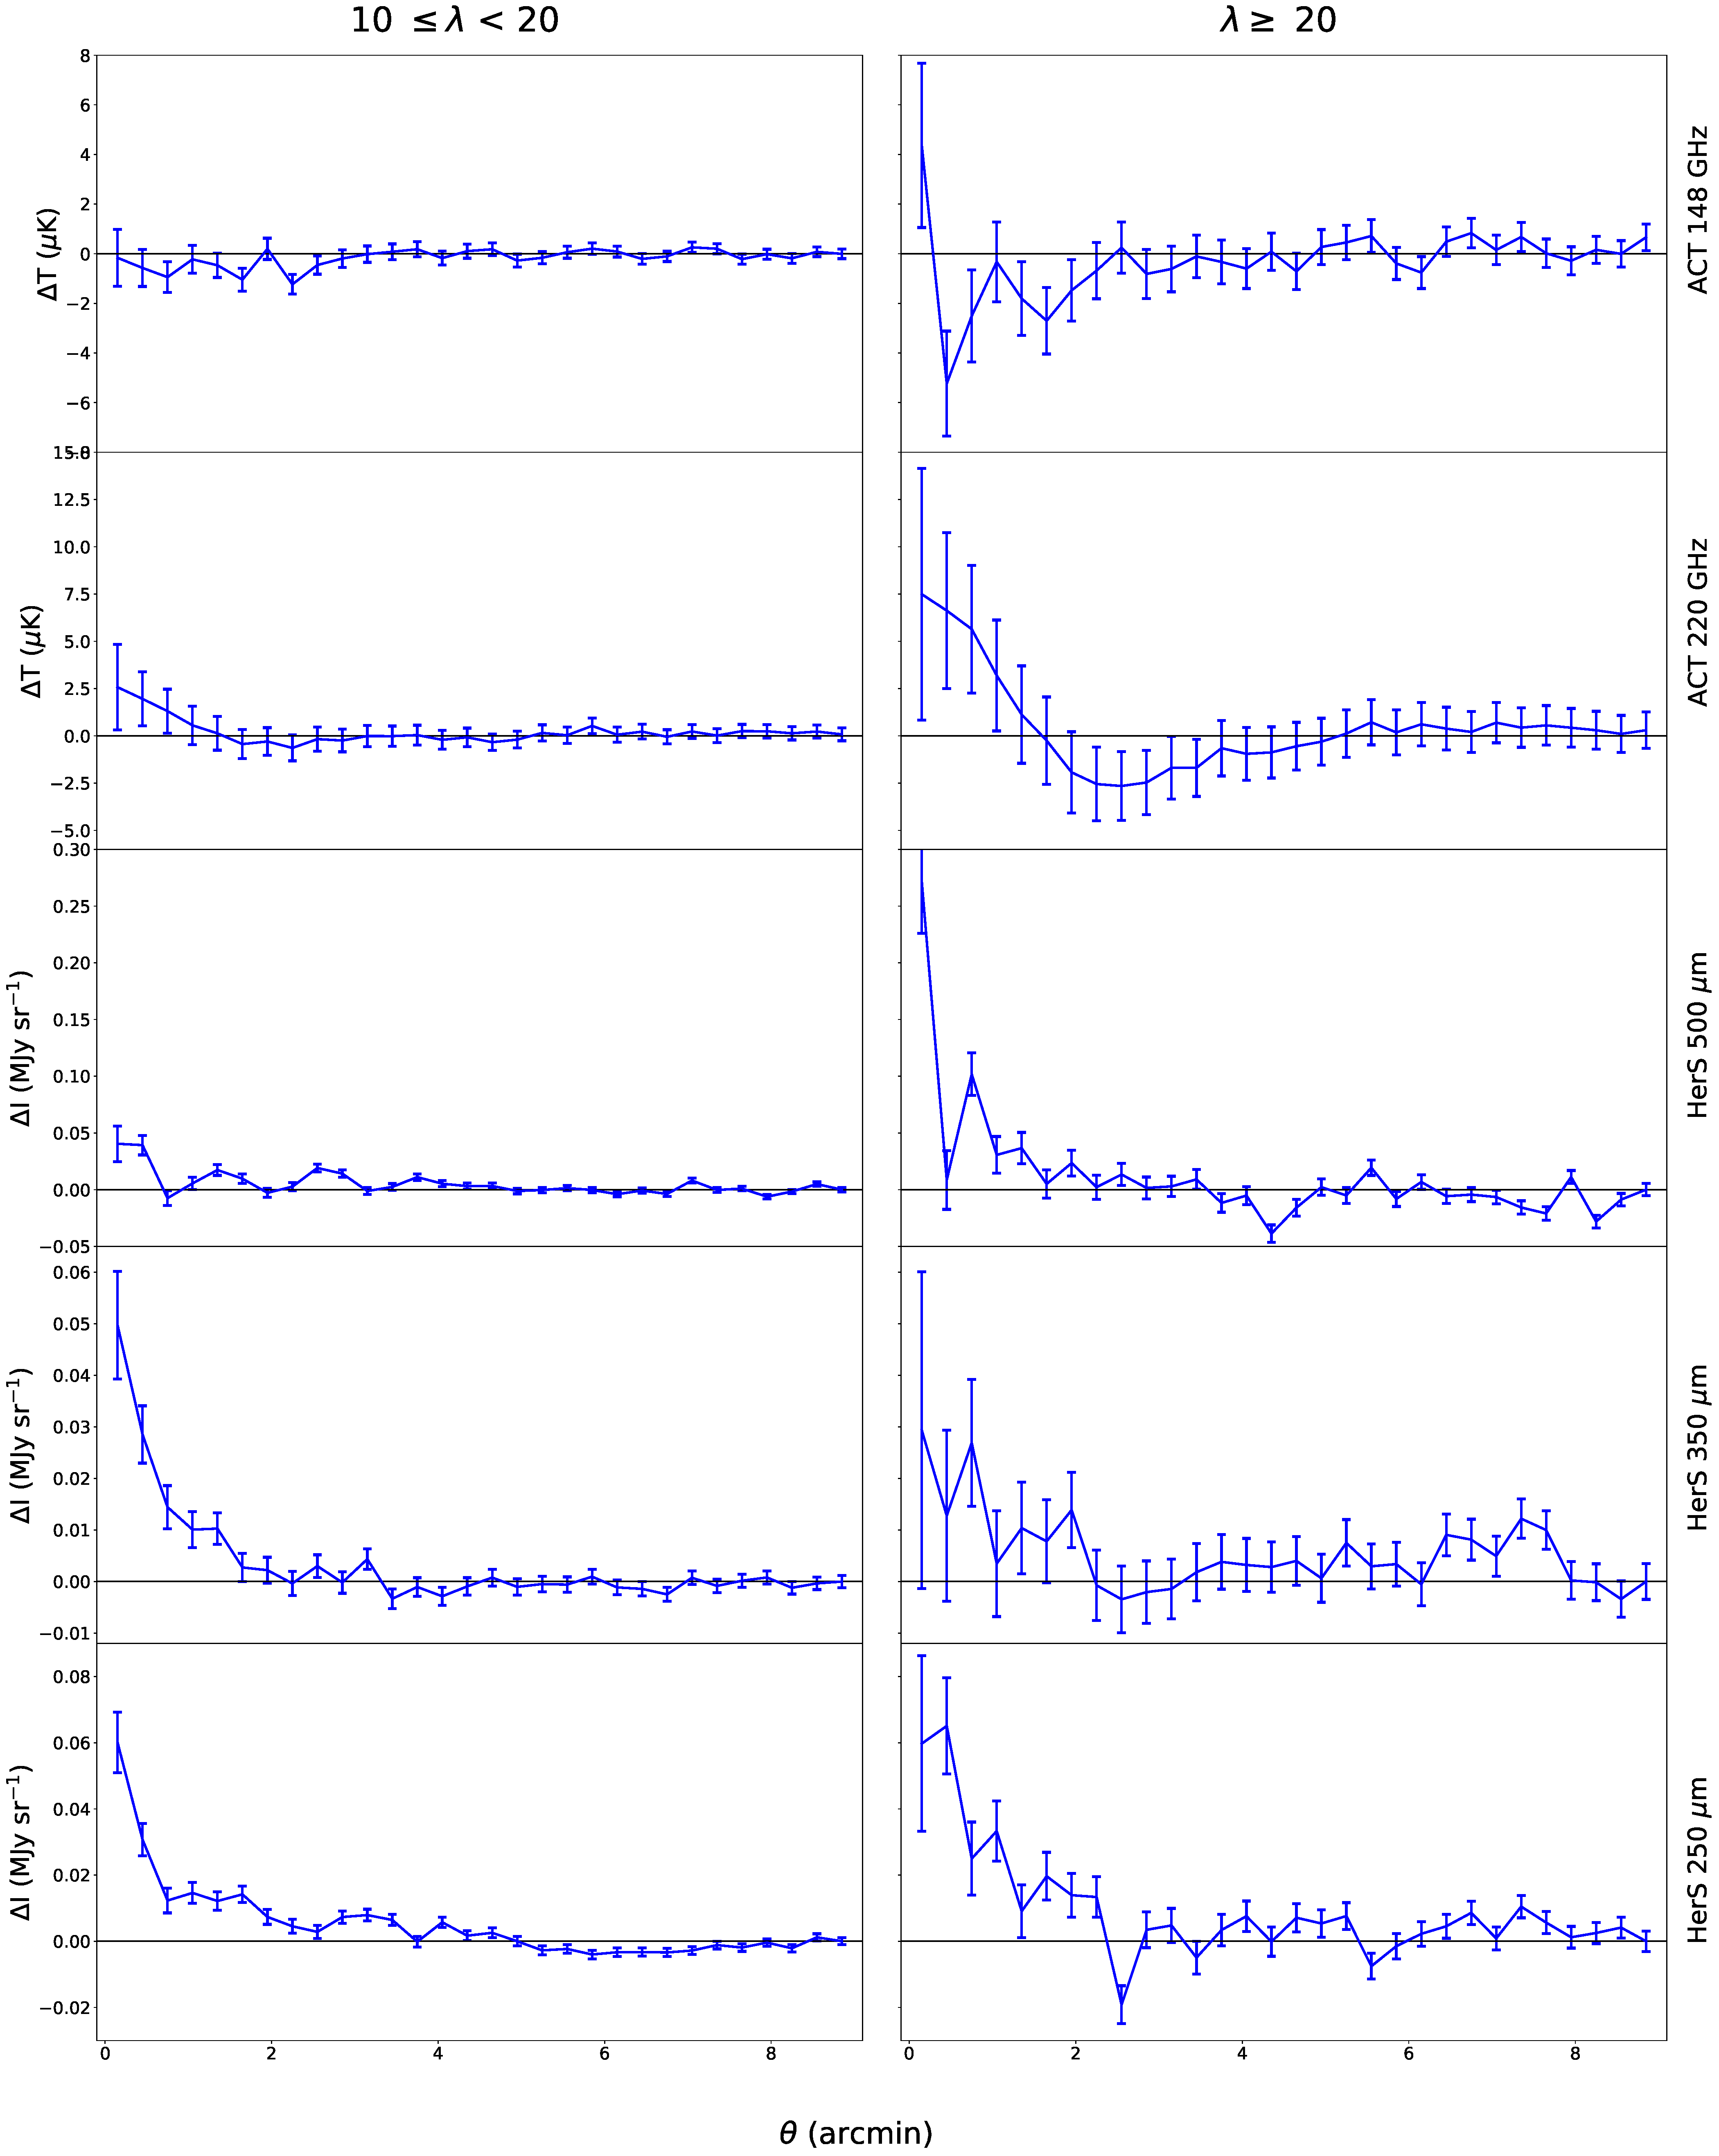
\includegraphics[height=0.9 \textheight]{5panel_rawprofs_all_stacks_all_ncut.pdf}

\caption{Stacked profiles for all 5 bands used in this analysis for the two richness bins: ACT 148, 220 GHz and HerS 500, 350, 250 $\mu m$. The main contributions to the profile at 148 GHz are the SZ signal, plus some signal from thermal dust emission. 220 GHz is near the SZ null, and contains emission which contaminates the signal at 148 GHz. The Herschel bands (500, 350, 250 $\rm \mu m$) trace thermal dust emission in the clusters. There are 623 clusters in the lower richness bin, and 75 in the higher.}  
  \label{fig:rawstacks}
\end{figure*}

\begin{figure}
  \centering
  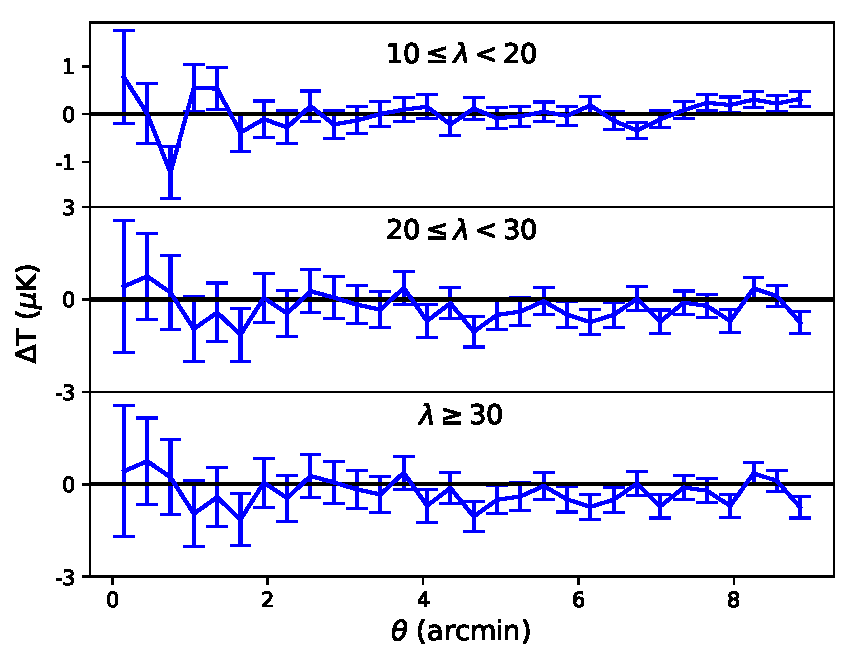
\includegraphics[width=0.5\textwidth]{rand_stacks_tophat.pdf}

\caption{Stacking null test at 148 GHz. Random positions for the number of clusters in each richness bin are stacked on to test that there is no SZ signal in places unassociated with clusters.}  
  \label{fig:randstacks}
\end{figure}




The stacked profiles for the two richness bins are shown in Figure \ref{fig:rawstacks}. The profiles from ACT at 148 and 220 GHz are shown as well as the profiles from stacking on the HerS maps. The profiles at 148 GHz exhibit the decrement associated with the SZ effect at frequencies below 218 GHz. Around 218 GHz is the SZ null, and the stacks at 220 GHz contain little SZ signal. They do contain cluster-centered emission, a fraction $\alpha_{\rm true}$ of which will also be present at 148 GHZ, as well as CMB and noise. We will use this 220 GHz emission profile as a template to clean the 148 profile and estimate the true SZ signal. Also shown are profiles from stacking on the HerS maps at 500, 350, and 250 $\mu$m. The HerS stacks are shown for reference; we did not use them when fitting for a dust spectrum. Instead, we used the band-merged source catalog \citep{2014ApJS..210...22V} to estimate $\alpha_{\rm true}$. The error bars on the stacked profiles result from stacking on the noise maps provided with the HerS data. The 220 GHz and Herschel stacks demonstrate that there is a signal from thermal dust emission within a few arcminute radius of the cluster centers.
To test that our signal is not only a feature caused by the stacking procedure we stack on random positions in the ACT map, finding no signal on average. Figure \ref{fig:randstacks} shows the results from stacking on random positions in the 148 GHz map, with each null stack accounting for the number of clusters in the different richness bins. The probability for $\chi^2$ to exceed the null hypothesis is 0.589 and 0.140 for the lower and higher richness bin random null stacks.


\subsection{Dusty Source Contamination}

Emission from dusty sources and radio sources is a contaminant of the SZ signal \citep{2005A&A...439..901A}. As seen in Figure \ref{fig:rawstacks}, when stacking at 220 GHz (the SZ null) there is an excess signal, which we attribute to dust emission from cluster member galaxies. This positive emission will also be present at 148 GHz, where it fills in the SZ decrement, effectively causing the sample to appear less massive. To correct for this, we use our 220 GHz stack as a template shape for dust contamination in the 148 GHz SZ signal, accounting for the different beam. We extrapolate the amount of emission in the 220 stack to 148 GHz by determining the dust SED of sources near the clusters and calculating the ratio of the flux density at 148 relative to 220, which we denote as $\alpha$. To determine $\alpha$, we fit a graybody SED to sources from the HerS survey that are near to the clusters. We also look at the correlation in the CIB power spectra at 143 and 217 GHz from Planck, which gives us a similar result. 
After applying the correction for dust, the profile at 148 GHz becomes:
\begin{equation}
\begin{split}
  P^{\rm corr,148} = b^{148} \ast \{ P^{\rm SZ} 
+ (1 - \alpha) n^{\rm CMB} + (\alpha_{\rm true} - \alpha) P^{\rm dust} \} 
\\+ n^{\rm det,148} - b^{148}( b^{220})^{-1} \ast \alpha n^{\rm det,220} 
  \end{split}
\end{equation}

%The covariance at 220 GHz does not take the CMB into account, so that contribution is not subtracted from the covariance %% THIS IS NO LONGER TRUE? - KMH

First, using the source catalog from the HerS survey \citep{2014ApJS..210...22V}, we fit a graybody SED 
\begin{equation}
  \label{eq:dustSED}
  \centering
  S(\nu) = A_{\rm dust}  \bigg(\frac{\nu(1+z)}{\nu_0}\bigg)^{\beta} \frac{\big(\nu(1+z)\big)^{3} }{{\exp({h \nu (1+z) / k T_{\rm dust}}) - 1}}
\end{equation}
for an overall amplitude, $A_{\rm dust}$, and dust temperature, $T_{\rm dust}$, using the total contribution of all the sources within a fixed angular distance from the clusters. We fix the emissivity spectral index $\beta$ to 1.5, $\nu_0$ to 100 GHz, and the redshift to the average redshift for each of the richness bins. \cite{2014A&A...561A..86M} find that setting $\beta$ to 1.5 is a good estimate when fitting spectra without enough information to constrain it, and note that it may cause $T_{\rm dust}$ to be slightly overestimated. Furthermore, when fitting for a stacked SZ plus greybody spectrum, \cite{2017arXiv170901187E} found that the choice of $\beta$ had little influence on the measured SZ signal, and use $\beta$ = 1.5 to obtain their main results. We ran our pipeline using $\beta$ = 1.4 and 1.6 to see how $\beta$ affects our results. For the lower richness bin, there was no change in the mass measurement. For the higher richness bin, $\beta$ = 1.4 increased the mass by 0.11$\sigma$, and $\beta$ = 1.6 decreased the mass by 0.06$\sigma$. To test whether the angular aperture within we include sources affects our SED measurement, we fit the spectrum to sources within a range of apertures.  We also tested whether fixing a reasonable value for $T_{\rm dust}$ and fitting for an amplitude and redshift affects the results. Including sources out to varying radii, between 1 and 11 arcminutes from the cluster center, we see similar 220 to 148 GHz extrapolation parameter $\alpha$. Fixing $T_{\rm dust}$ and allowing the redshift to vary also gives a similar extrapolation, both fitting methods result in realistic values for $T_{\rm dust}$ or $z$. The only information we need is the SED between 220 and 148 GHz, which is used to calculate $\alpha$. This is given by the shape of the dust SED, meaning the exact fitted values for the amplitude, $T_{\rm dust}$, or $z$ are not as important to the analysis as long as they are realistic. 
We report results fitting sources with an 11' aperture in Table \ref{table:mcmcfitparam}. We find a value of 0.28 for $\alpha$, meaning that 28\% of the emission present in the stacked profile at 220 GHz is carried over to 148 GHz.

\begin{equation}
\mathcal{D}_{\ell}^{\rm CIB_{143 \times 143}} = A^{\rm CIB}_{143} \bigg(\frac{\ell}{3000}\bigg)^{\gamma^{\rm CIB}}, \quad
\mathcal{D}_{\ell}^{\rm CIB_{217 \times 217}} = A^{\rm CIB}_{217} \bigg(\frac{\ell}{3000}\bigg)^{\gamma^{\rm CIB}},
\end{equation}
which are translated to ACT frequencies using:
\begin{equation}
\mathcal{D}^{\rm CIB_{\nu_{i} \times \nu_{j}}}_{\ell} = \mathcal{D}^{\rm CIB_{\nu_{i0} \times \nu_{j0}}}_{3000} \bigg( \frac{g(\nu_{i})g(\nu_{j})}{g(\nu_{i0})g(\nu_{j0})} \bigg) \bigg( \frac{\nu_{i} \nu_{j}}{\nu_{i0} \nu_{j0}} \bigg)^{\beta_{\rm d}} \frac{B_{\nu_{i}}(T_{\rm d})}{B_{\nu_{i0}}(T_{\rm d})} \frac{B_{\nu_{j}}(T_{\rm d})}{B_{\nu_{j0}}(T_{\rm d})}
\end{equation}
\newline 
where $B_{\nu}(T_{\rm d})$ is the Planck function, $g(\nu) = [\partial B_{\nu}(T)/\partial T]^{-1}|_{T_{\rm CMB}}$, and the parameters $\beta_{\rm d}$ and $T_{\rm d}$ are fixed at 2.20 and 9.7 K, respectively.
We then use the ratio in the power spectra to convert our 220 signal into a correction for the 148 GHz stack. We find with this method that 28 $\pm$ 7\% of the signal at 220 is carried over into the 148 stack, in agreement with the value of $\alpha$ we found from the Herschel fitting.



\subsection{Radio Source Contamination}
Radio sources have been found to preferentially reside in clusters of galaxies and are often associated with emission from the cluster member galaxies \citep{2002ApJ...580...36H,2007ApJS..170...71L,2007AJ....134..897C,2009ApJ...694..992L}. Similarly to the process of measuring dust emission, we look for radio sources within 11' and model their emission at 148 and 220 GHz. We use sources from the NVSS survey at 1.4 GHz \citep{1998AJ....115.1693C}. We find no bright sources within this sample after our initial pruning, and extrapolate the stacked synchrotron emission profile using spectral indices $-0.5$, $-0.7$, and $-0.9$. We find emission in the ACT bands that is much lower than the SZ signal, and therefore we make no further correction.



\section{Results} \label{sec:results}

We use a Monte Carlo formalism to fit for $M_{500}$ from our stacked profile at 148 GHz. We then use richness information available from the IR and optical data to compare to other works.



%%%%%%%%%%%%%%%%%%%%%%%%%%%%%%%
%RESULTS
%%%%%%%%%%%%%%%%%%%%%%%%%%%%%%%

\subsection{Mass Fitting}

\begin{table*}
   
  \centering
  \caption{Best-fit parameters for fitting an SZ profile in two ways: correcting for dust emission, and neglecting dust contamination.}
  \begin{threeparttable}
  \begin{tabular}{|*{7}{c|}}
    \hline
    & & \multicolumn{2}{|c}{$10 \leq \lambda < 20$} & & \multicolumn{2}{|c|}{$\lambda \geq 20$} \\ \hline
    
    & & Dust corr. & No dust corr. & \ &  Dust corr. & No dust corr.  \\ \hline
    
    $M_{500}$ (10$^{13}$ M$_{\odot})$ & & $1.7 \pm 0.8$ & $0.88 \pm 0.52$ & \ & $4.9 \pm 1.7$  & $2.2 \pm 1.1$ \\ \hline
    
    $p_0 \ (\rm \mu K)$ & & $-0.09 \pm 0.13$ & $-0.18 \pm 0.26$ & \ & $0.07 \pm 0.32$ & $0.14 \pm 0.66$ \\ \hline
    
    $A_{\rm dust} \ (\rm 10^{14} Jy/Hz^3)$ & & $1.19 \pm 0.08$ & - & \ & $1.55 \pm 0.29$ & - \\ \hline
    
    $T_{\rm dust} \ (\rm K)$ & & $29.1 \pm 0.1$  & - & \ & $27.2 \pm 0.2$ & - \\ \hline \hline
    
    $\alpha$ & & $0.2806 \pm 0.0002$ & - & \ & $ 0.2812 \pm 0.0002 $ & - \\ \hline
    
    \end{tabular}
  \begin{tablenotes}
	\item Resulting fit parameters for the two richness bins. The first column for each richness bin shows results from fitting for a dust SED simultaneously with the SZ profile to remove dust emission, fixed at the average redshift for each sample (for $1-b=1$). The second column lists the results if we neglect the dust correction (for $1-b=1$) and fit an SZ profile directly to the original stacked profile. The distribution for $\alpha$ is not sampled in the MCMC chains, but is calculated using $A_{\rm dust}$ and $T_{\rm dust}$.
  \end{tablenotes}
  \end{threeparttable}
\label{table:mcmcfitparam}
\end{table*}


To take into account how the dust correction affects the mass fitting, we simultaneously fit for a dust SED and an SZ profile. We use a Gaussian likelihood and the affine-invariant Markov Chain Monte Carlo code \textit{emcee} \citep{2013PASP..125..306F}. The fit parameters are the average cluster mass $M_{500}$, an overall DC offset for the stacked profile $p_0$, an amplitude for the graybody SED $A_{\rm dust}$, and a dust temperature $T_{\rm dust}$. We fix the redshift dependence of the dust spectrum and SZ signal to the average redshift for each sample, z = 0.80 and 0.71, for the lower and higher richness bins. We apply a flat prior for values within the following ranges: $0 M_{\odot} <  M_{500} < 10^{15} M_{\odot}$,$\ -10 \mu$K $< p_0 < +10 \mu$K, 0 mJy/Hz$^3$ $< A_{\rm dust}$ < 0.1 mJy/Hz$^3$,$\ 3 $K $< T_{\rm dust} < 500$K. 
The HerS flux densities are used to sample the graybody SEDs. The ratio of the SED at 148 and 220 GHZ is used to calculate $\alpha$, which gives our dust correction by allowing us to extrapolate the 220 GHz profile to 148 GHz, assuming that the profile at 220 GHz is dominated by dust emission. The extrapolated dust signal is subtracted from the raw stack at 148 GHz.
The UPP with updated parameters is integrated to calculate the SZ signal $y(\theta)$, which is convolved with the ACT beam and translated into a temperature profile, $\Delta T(\theta)$, that is fit to our dust-subtracted stacked profile. 


\begin{figure}
  \centering
  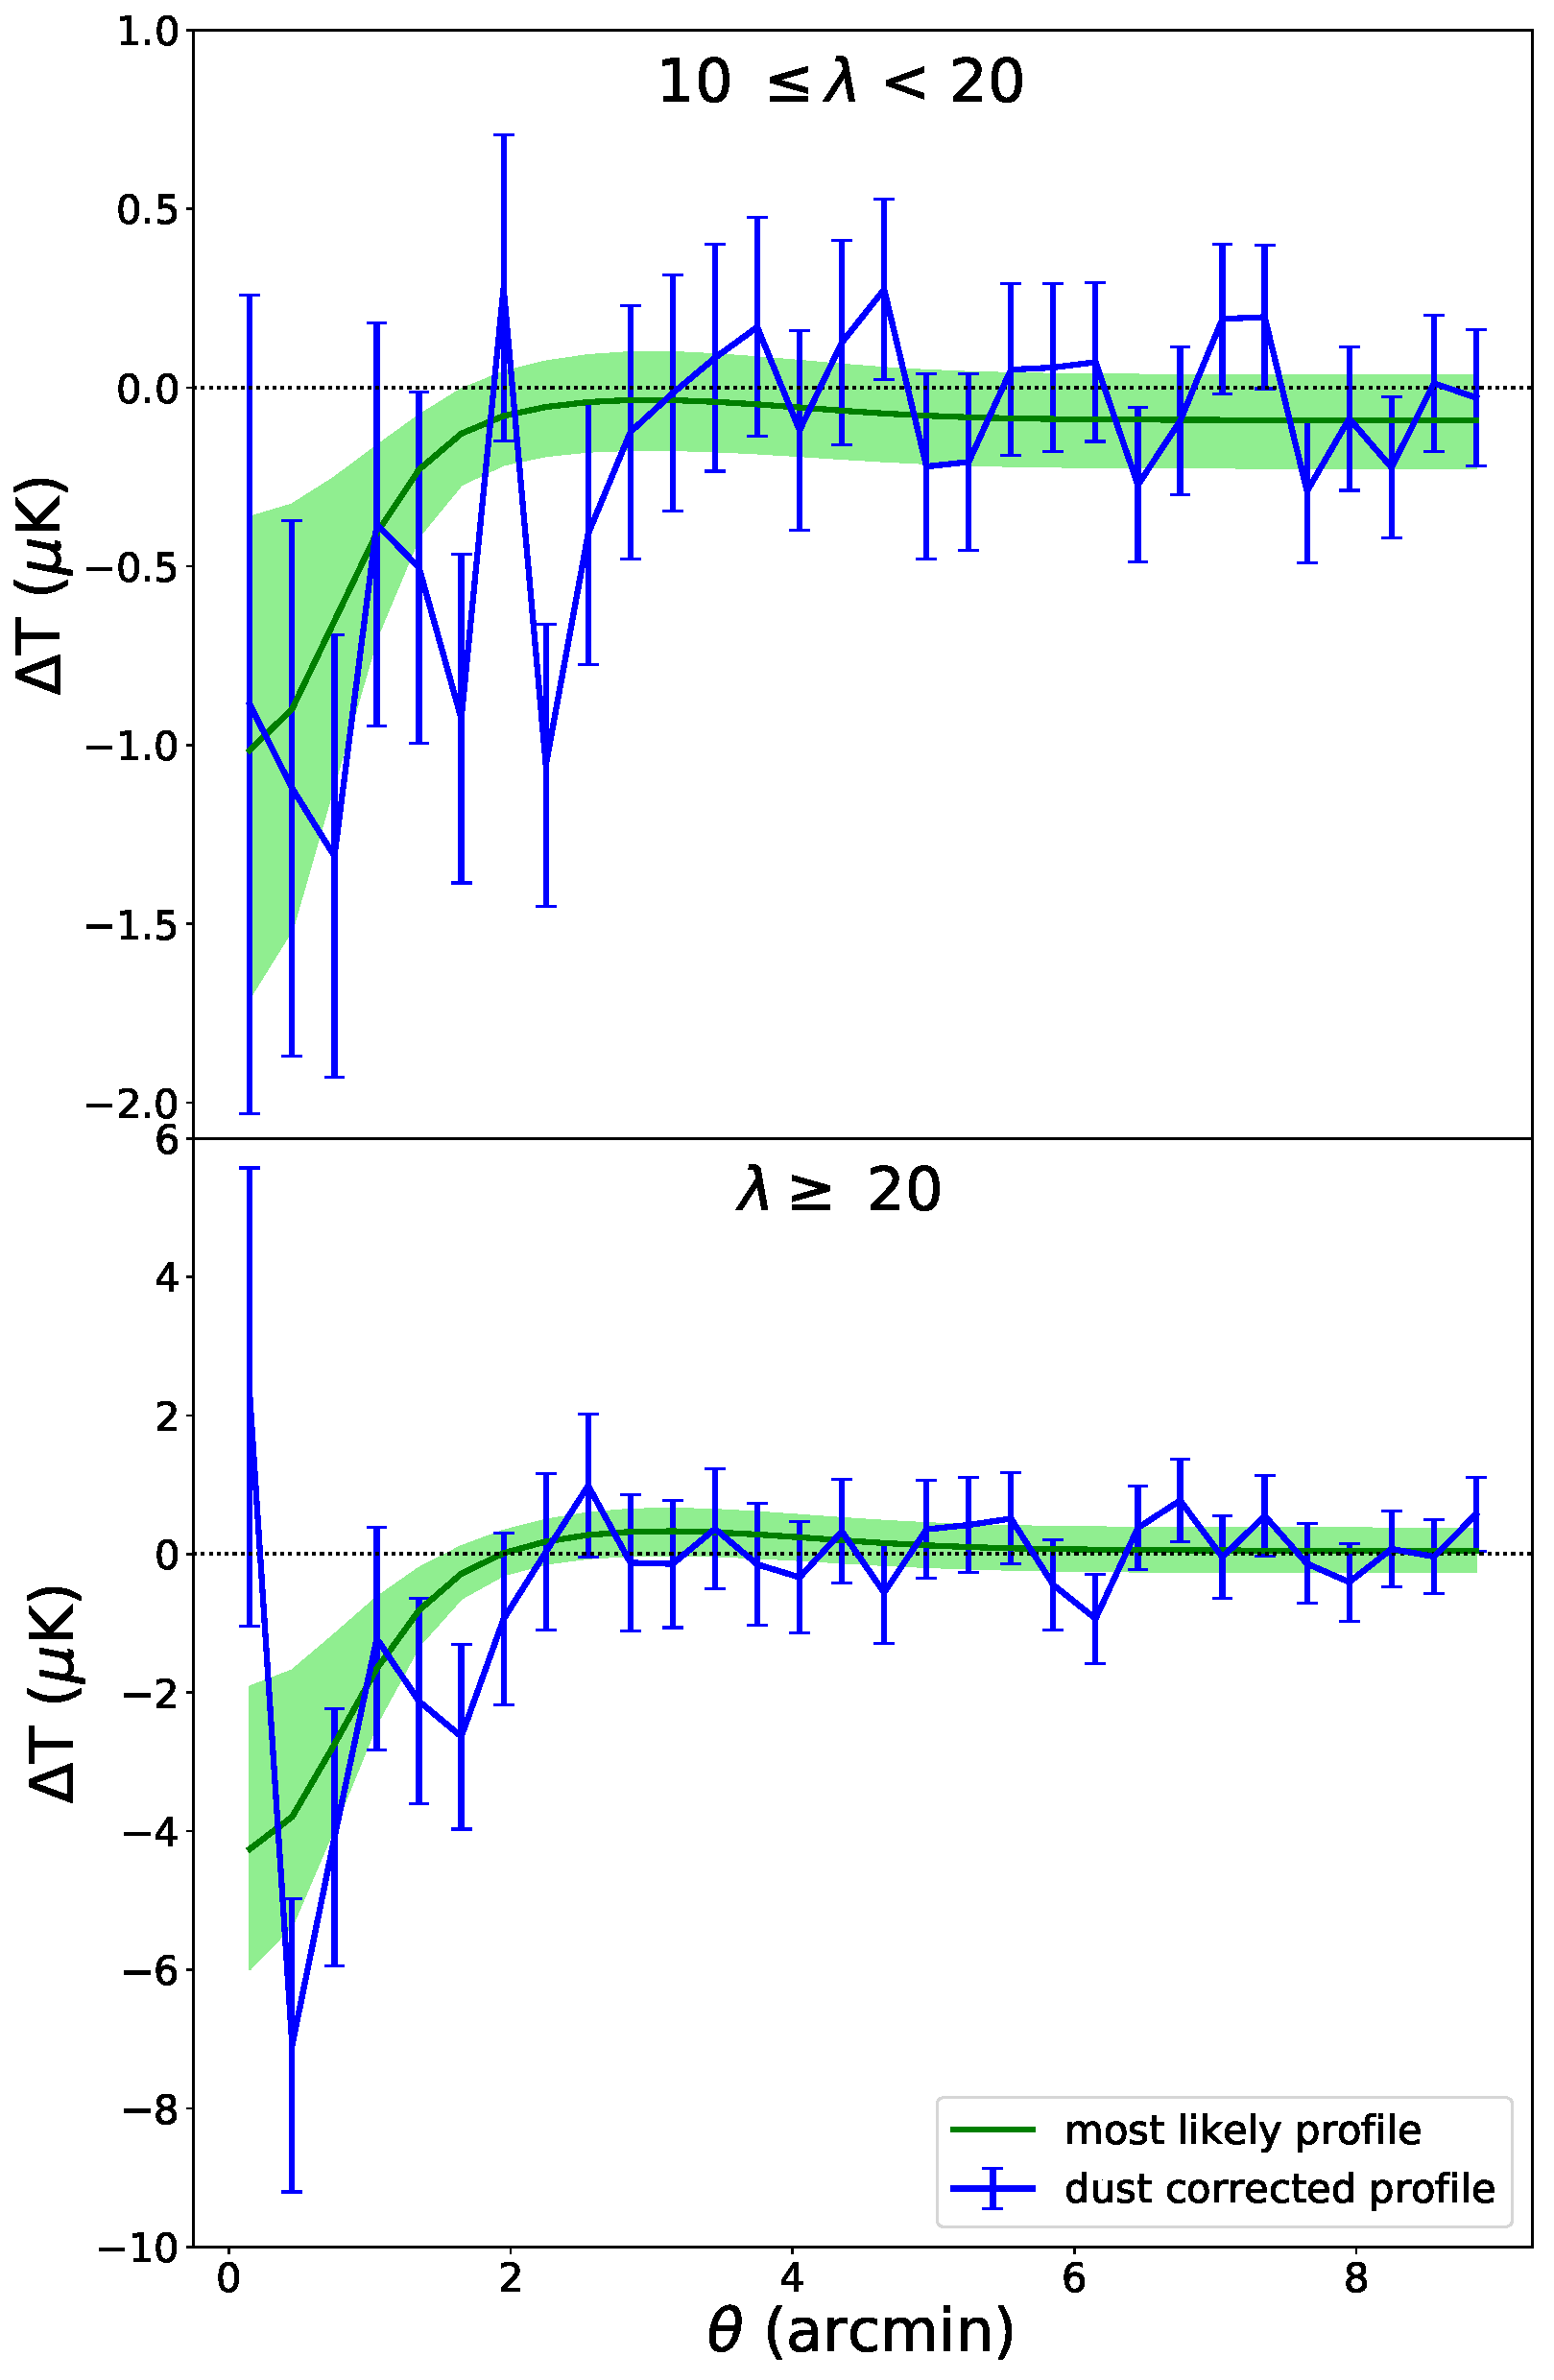
\includegraphics[width=0.5 \textwidth]{MLprof_ncut_all.pdf}
  \caption{Results from fitting for a cleaned SZ profile for the three richness bins. The blue line is the stacked profile after taking into account the dust correction, given by $\alpha$ and the profile at 220 GHz. The green line is the result from the MCMC chains. The green contours bound the models in the chain between the 16th and 84th percentiles in each angular bin.}
  \label{fig:mcmcprof}
\end{figure}


%%%%%%%%%%%%%%%%param contours



\begin{figure}
  \centering
  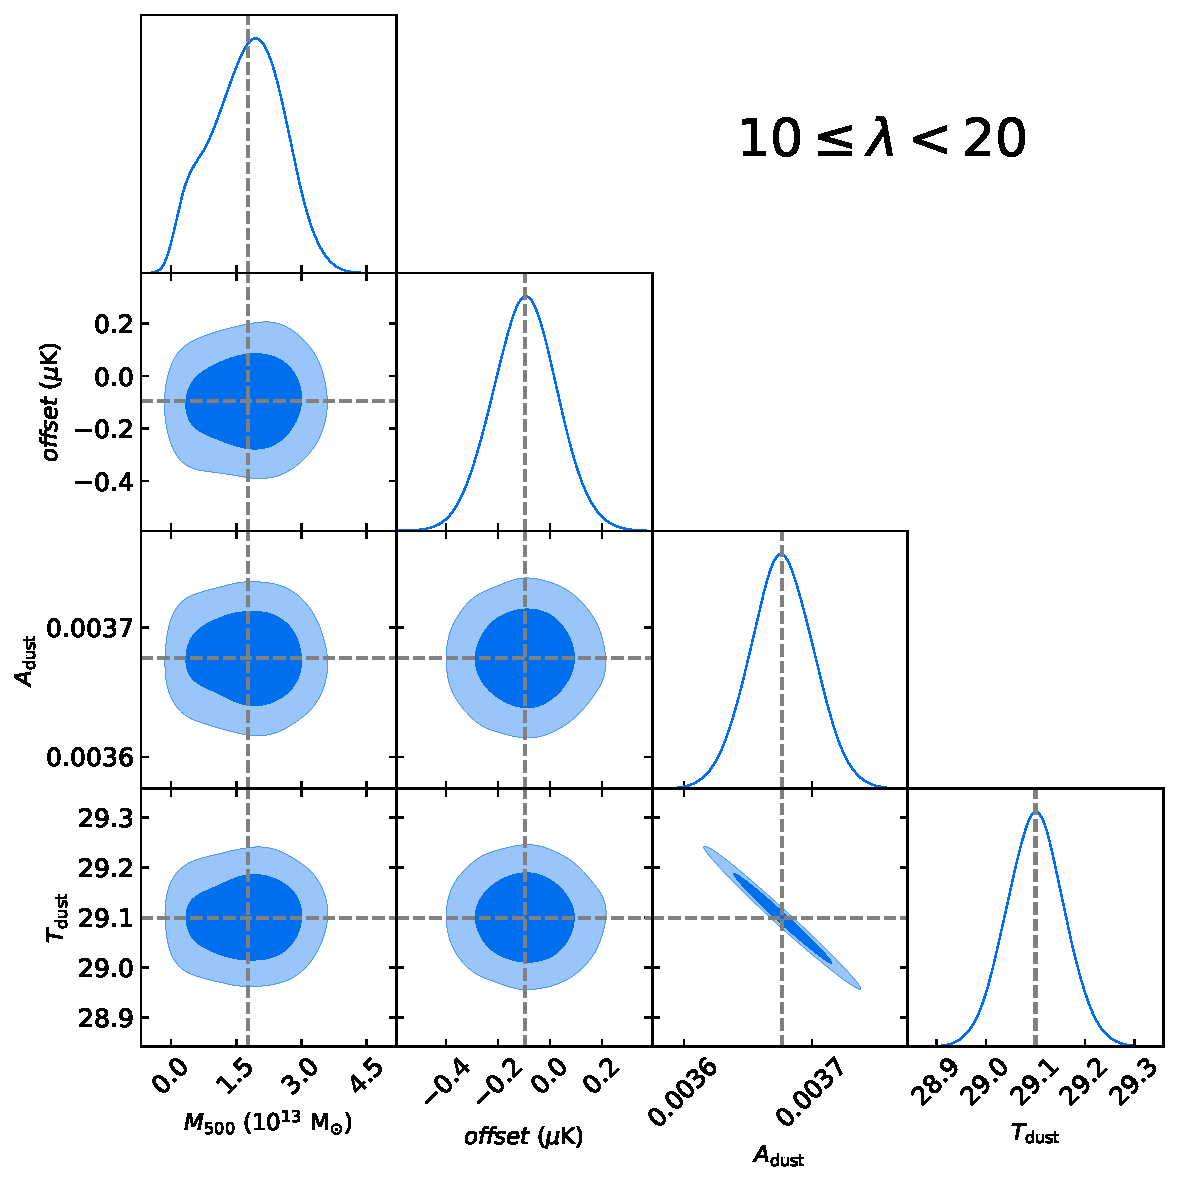
\includegraphics[width= \columnwidth] {corner_171219_nw_12_ns_10000_mbat_tophat_11_arcmin_ncut_10_20_cut_1000.pdf}
  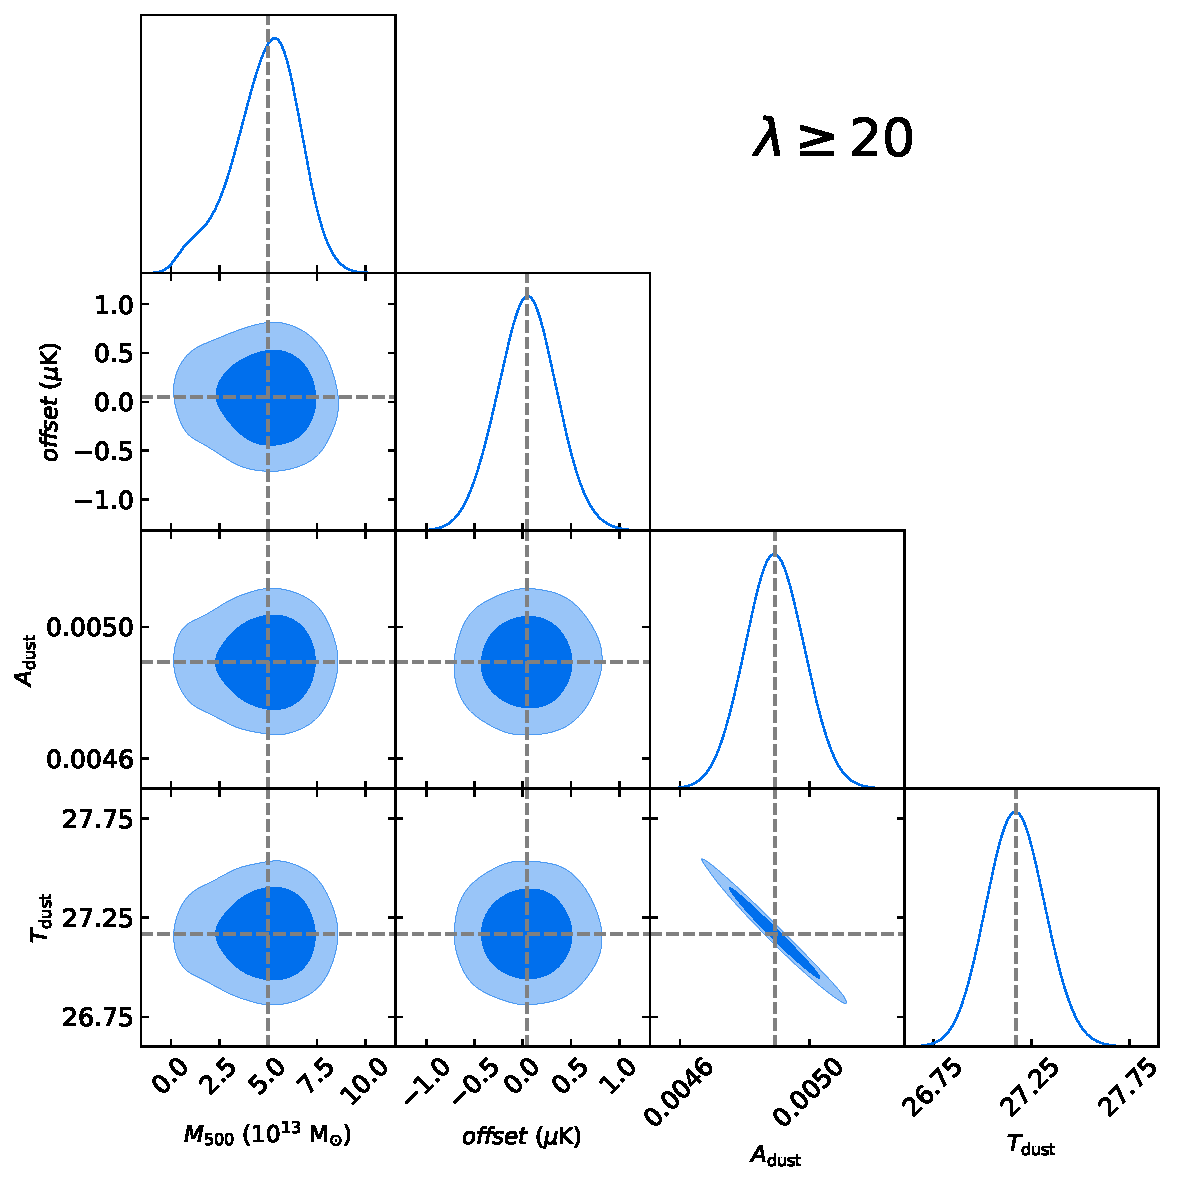
\includegraphics[width= \columnwidth] {corner_171219_nw_12_ns_10000_mbat_tophat_11_arcmin_ncut_gt20_cut_1000.pdf}
  \caption{Parameter contours from MCMC chains for the lower (top) and higher (bottom) richness bins. The grey dashed lines pass through the mean value from the probability distributions for each parameter. The dust amplitude and temperature are anti-correlated in both richness bins.}  \label{fig:mcmccontours}
\end{figure}

%leave this out but mention when describing earlier plot
%\begin{figure*}
%  \centering
%  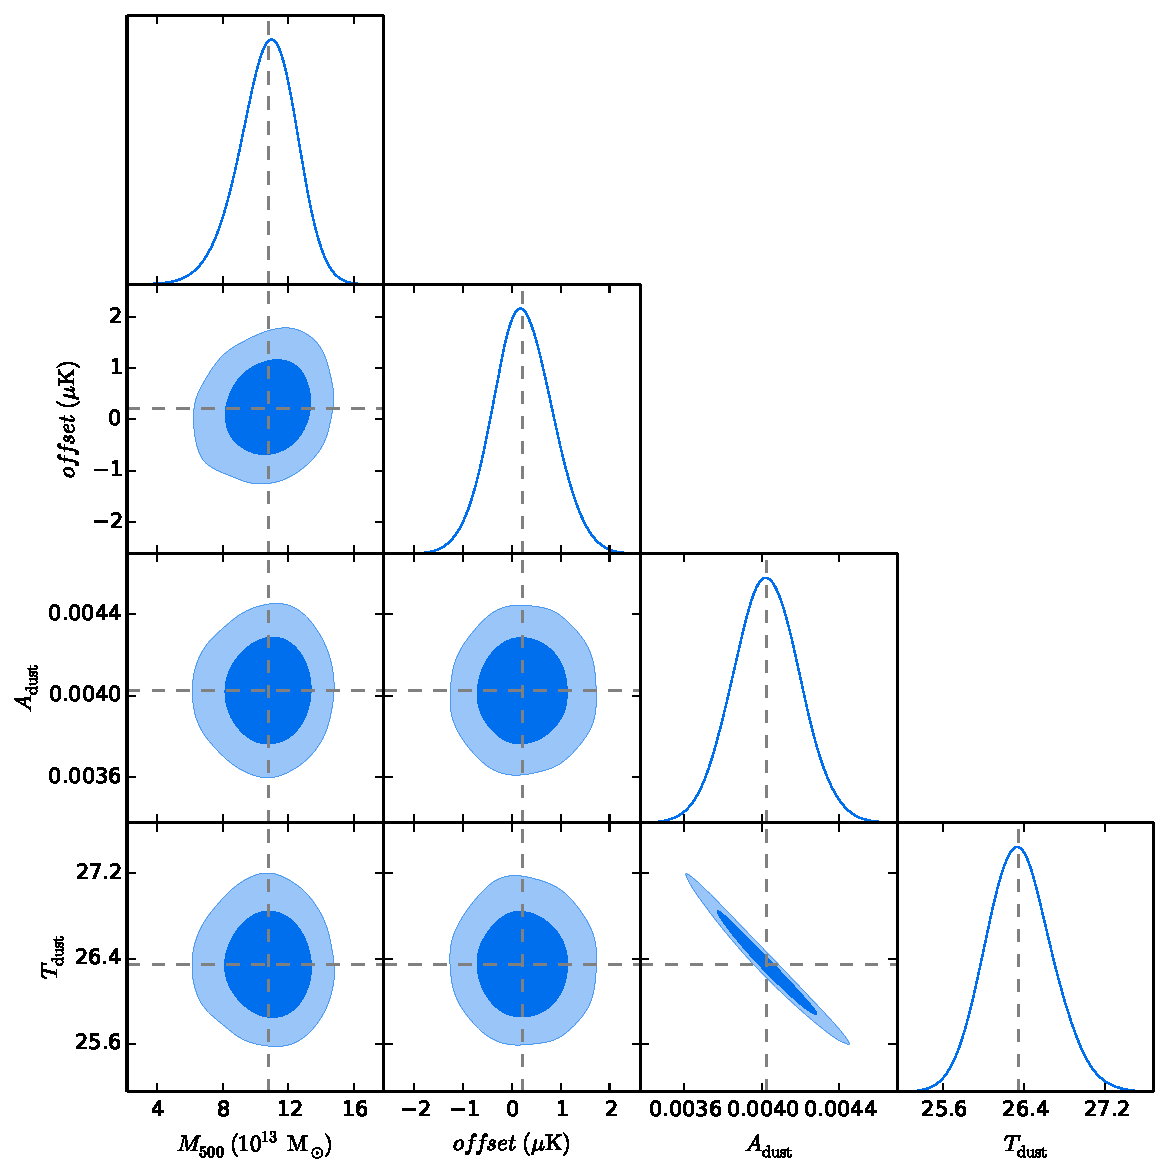
\includegraphics[width= \textwidth] {corner_1212_nw_12_ns_10000_mbat_11_arcmin_cut_161005_ncut_30_cut_1000.pdf}
%  \caption{Parameter contours from MCMC chains.  } %\label{fig:mcmccontours}
%\end{figure*}






Figures \ref{fig:mcmcprof} and \ref{fig:mcmccontours} show the results from fitting the stacked profile and IR data to a dust SED and cleaned SZ profile. Figure \ref{fig:mcmcprof} shows the cleaned SZ profiles along with the most likely profiles from the MCMC chains. The light green area encompasses 68\% of the models from the MCMC chains in each bin.  For both richness bins, Figure \ref{fig:mcmccontours} shows the parameter contours for $M_{500}$, redshift, a DC offset in the 148 GHz stack, a dust spectrum amplitude, and a dust temperature from the MCMC chains. The lower tails of the distributions for $M_{500}$ are pushing against the prior, which is zero. None of the parameters seem correlated except the dust amplitude and temperature, which are anti-correlated. 
The fit parameters are summarized in Table \ref{table:mcmcfitparam}, which show results from simultaneously fitting a dust SED and SZ profile to the stacked 148 GHz data and fitting an SZ profile directly to the data while correcting and neglecting to correct for dust. Neglecting to correct for dust decreases the mass by a factor of 0.53 for $10 \leq \lambda < 20$, and a factor of 0.45 for $\lambda \geq 20$. %In terms of the SZ signal $Y_{500}$, only 38\% and 29\% of the signal would be measured without accounting for dust contamination. 
We use the random stacks from Figure \ref{fig:randstacks} to test what mass our pipeline measures when there is no signal. Fitting without a dust correction results in probabilities of measuring the mass that pushed up against the lower limit of the prior, zero. At 95\% confidence, the upper limit of the distributions are 2.0 $\times 10^{13} M_{\odot}$ and 3.1 $\times 10^{13} M_{\odot}$, for the lower and higher richness bins. These masses measured for the lower richness bin are close to the values measured in the main analysis, showing that there is only evidence of the SZ signal for these clusters. 
When also measure the SZ mass of only the dust correction, using the data stack at 220 GHz as shown in Figure \ref{fig:rawstacks} (the case of zero SZ signal), and measure masses of $(1.6 \pm 0.8) \times 10^{13} M_{\odot}$ and $(2.7 \pm 1.6) \times 10^{13} M_{\odot}$ for the lower and higher richness bins respectively. In terms of $Y_{500}$, this means that 80\% $\pm$ 65\% of the SZ signal in the lower richness bin and 65\% $\pm$ 40\% of the SZ signal in the higher richness bin is filled in by dust emission. Figure \ref{fig:y500dist} shows the probability distributions of measuring $Y_{500}$ for these two cases, and is meant to show how the probabilities are distributed and show that the dust correction makes a large portion of the measured SZ signal. 


\begin{figure}
  \centering
  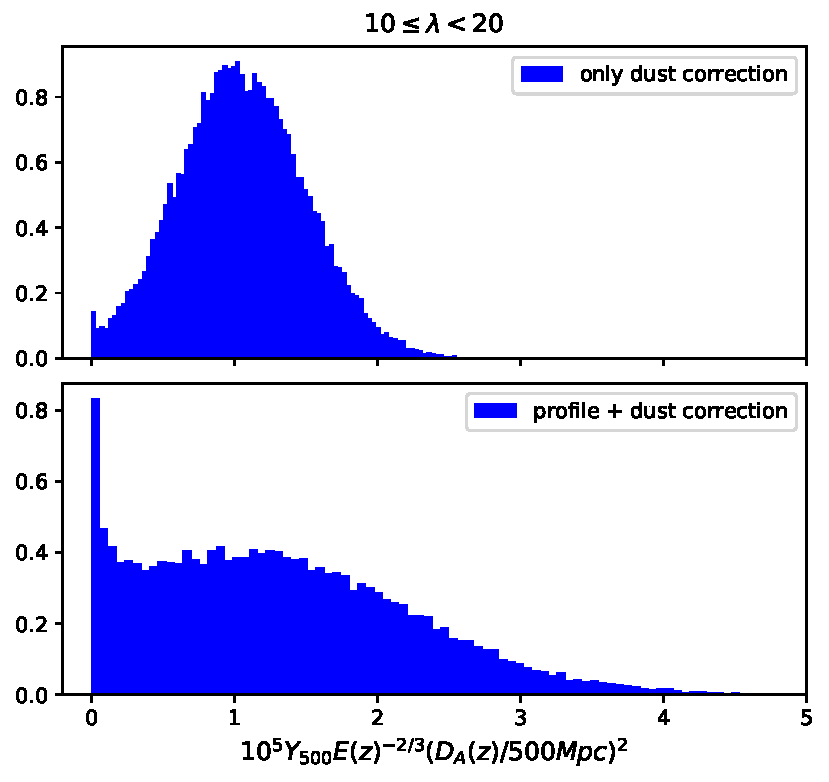
\includegraphics[width= \columnwidth] {chains2y500_10_20.pdf}
  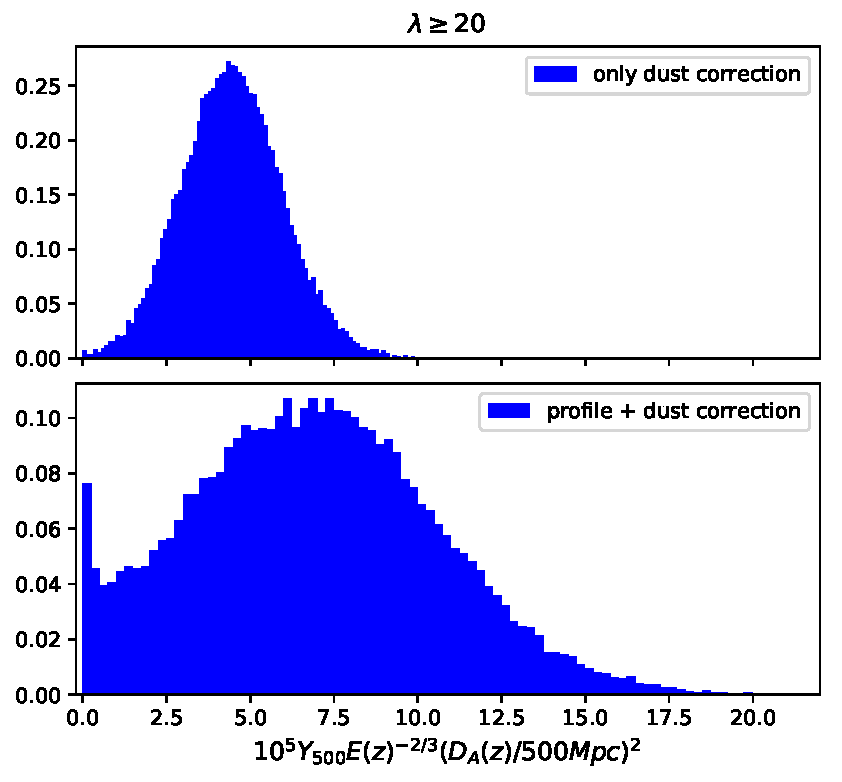
\includegraphics[width= \columnwidth] {chains2y500_gt20.pdf}
  \caption{Probabilities of measuring $Y_{500}$ for two different cases, for each richness bin. The upper plots for each richness bin are the distributions for $Y_{500}$ of only the dust correction (the case of no signal at 148 GHz). The lower plots for each richness bin are the distributions of $Y_{500}$ for the dust corrected stacked profiles. For both richness bins, it can be seen that the dust correction is a significant portion of the total mass measurement.}  
  \label{fig:y500dist}
\end{figure}




\subsection{Mass Bias}



The relation between SZ signal and cluster mass, $Y$--$M$, is measured using x-ray derived cluster masses \citep{2010A&A...517A..92A, 2011ApJ...738...48A}, but there are several effects that cause these x-ray mass measurements to be biased low. Clusters are assumed to be in hydrostatic equilibrium (HE), but non-thermal pressure support from turbulence and random motions move the clusters away from perfect HE. Single temperatures are also fit to x-ray data, but subregions with higher temperatures can be present and get averaged down, resulting in a bias toward measuring a lower temperature and therefore mass. The bias between the true mass and the mass measured by the SZ effect is $1-b = M/M_{\rm true}$. The precise value for $1-b$ is not well understood and could have a large range of values\citep{2014A&A...571A..16P}. In \cite{2014A&A...571A..16P}, $1-b$ is fixed at 0.8 as an estimation of the possible value. \cite{2016JCAP...08..013B} measured the mass bias for high signal to noise clusters from the ACT equatorial survey, using weak-lensing data from the Canada-France-Hawaii telescope stripe 82 survey. They found that $1-b$ is 0.98 $\pm$ 0.28 and 0.87 $\pm$ 0.27 when fitting the weak-lensing mass using models based on simulations and an NFW profile, respectively. There have been several other measurements of $1-b$, with values ranging from 0.58 to 0.95 \citep{2014MNRAS.443.1973V,2015MNRAS.449..685H,2016MNRAS.456L..74S,2016A&A...594A..24P}. When comparing our measured $M_{SZ}$ to cluster mass scaling relations, we use the values: $1-b = 1$, 0.8, and 0.6. We choose these values to sample the range of values that have been measured, so that we can demonstrate how much different amounts of hydrostatic mass bias could affect our mass measurements. 


\iffalse
\subsection{SZ-Mass Scaling Relations}

\subsubsection{Stellar Mass}

\begin{table}
  
  \centering
  \caption{Average stellar mass content for each subset of cluster candidates, with $1-b=1$.}
  \begin{threeparttable}
  \begin{tabular}{|*{4}{c|}}
    \hline
    & $10 \leq \lambda < 20$ & $20 \leq \lambda < 30$ & $\lambda \geq 30$ \\ \hline
	 $M^{\ast}_{500}$ (10$^{13}$ M$_{\odot})$ & $0.049^{+0.002}_{-0.004}$ & $0.165^{+0.015}_{-0.037}$ & $0.205^{+0.044}_{-0.059}$ \\ \hline
     $f^{\ast}_{500}$ & $0.028^{+0.0104}_{-0.0102}$ & $0.029^{+0.0085}_{-0.0062}$ & $0.019^{+0.0064}_{-0.0052}$ \\ \hline
    
    \end{tabular}
%  \begin{tablenotes}
%	\item \textbf{this needs to be updated}
%  \end{tablenotes}
  \end{threeparttable}
\label{table:stellarmass}
\end{table}

Galaxy clusters are good samples of the matter content of the universe. Understanding the baryon content of galaxy clusters is important as it tells us about physical mechanisms at play, and is a test for models of cluster galaxy evolution. There have been several works mapping out the relation between halo mass and stellar mass, and as we have a data set which includes SZ, infrared, and optical data, we compare our data to those studies. 

For the SHELA sample, stellar mass measurements for the member galaxies of each cluster are obtained using FAST (Fitting and Assessment of Synthetic Templates) \citep{2009ApJ...700..221K} and photometric redshifts are obtained using EAZY \citep{2008ApJ...686.1503B}. FAST uses broadband photometry and photometric redshifts to fit the age, dust content, star formation timescale, metallicity, stellar mass, and star formation rate for each galaxy. We use the galaxy stellar masses from FAST along with the positions and galaxy cluster membership probabilities from the redMaPPer catalog to find the total stellar mass per cluster. We sum the stellar mass for each member galaxy weighted by its membership probability within a projected radius of $R_{500}$. $R_{500}$ is computed using $M_{500}$ from the SZ fitting and the average redshift for each richness bin. We then average the stellar masses for each cluster in the richness bin to obtain an average stellar mass out to $R_{500}$. Some of the clusters are missing stellar mass information, 24 clusters from the lower richness bin and 4 clusters from the higher bin. The results are summarized in Table \ref{table:stellarmass}, which reports the average stellar mass for each richness bin and $f^*_{500}$ --- the fraction of stellar mass to total mass within $R_{500}$. %We find a higher value for $f^*_{500}$ for the lower richness subset, $2.9^{+0.85}_{-0.37}\times 10^{-2}$, and $1.9^{+0.64}_{-0.52}\times 10^{-2}$ for the higher richness subset. For our data, the relation between stellar mass and halo mass is: $M^*_{500} \propto M_{500}^{s_1}$, where $s_1 = 0.35^{+1.41}_{-0.94}$. $f^*_{500} \propto M_{500}^{s_2}$, where $s_2 = -0.65^{+1.71}_{-1.34}$. As we only have two bins, neither slope is well-defined, but we compute them to compare to other works in the literature.

------
all log normal?

Hilton: Salpeter IMF, z range: 0.27 to 1.07, median 0.5, mass range: 2-14 e14 Msol, median 7e14 Msol. intrinsic scatter siglogm500 = 0.10 +- 0.06, how to invert? look at what i did for spt

Budzynski: Chabrier IMF, z range: 0.15-0.4, mass range:  5e13-1e15 Msol. Not sure what scatter is

Andreon: m/l Cappelari, z range: 0.03-0.1, mass range:5e13-1e15. intrinsic scatter (term left after accounting measurement err) sigmalogmstar = 0.15 +- 0.02 dex

Giodini: Salpeter, z range: 0.1-1.0, mass range:1e13-1e15 (a lot in 1e13-1e14 range). 35\% log scatter

van der Berg: Chabrier IMF, z range: 0.86-1.4, mass range: m200  mostly 7-12e13, one 1e15. intrinsic scatter sigmalogmstar = 0.11 +0.05-0.04 dex

!giodini/vdb in our mass range

------

%We find that our data agree with an inverse scaling between stellar and halo mass, but we find values for $f^*_{500}$ that are smaller than what is seen in other studies.
\cite{2013MNRAS.435.3469H} performed the first measurement of stellar masses for SZ-selected clusters. They studied 14 ACT SZ-selected clusters with dynamical masses ranging from $(2-14) \cdot 10^{14} M_{\odot}$. Their stellar masses came from Spitzer 3.6 and 4.5 micron imaging. They found a stellar mass fraction within $R_{500}$ ranging from 0.0006 to 0.034, which is higher than what we find, considering that they look at more massive clusters.
\cite{2013ApJ...778...14G} used a sample of optically-selected clusters with XMM-Newton data to study the relation between gas, stellar, and total mass in galaxy clusters. They found that $f^*_{500} \propto M_{500}^{-0.45 \pm 0.04}$, which the SHELA data is consistent with due to our large uncertainty.  
\cite{2010MNRAS.407..263A} used optical data to measure dynamical masses and stellar masses for a sample of groups and clusters, which overlap in mass with the SHELA sample. They found $f^*_{500} \propto M_{500}^{-0.55 \pm 0.15}$. At $log(M_{500}/M_{\odot}) = 13.76$ and 14.03, near the SHELA sample masses, they found that $f^*_{200} =$ 0.042 $\pm$ 0.0115 and 0.025 $\pm$ 0.011, which is higher than what we find in the SHELA data, but also takes into account the stellar mass out to $R_{200}$ instead of $R_{500}$. 
\fi

\subsection{Richness to Mass Scaling}

\begin{figure}
  \centering
    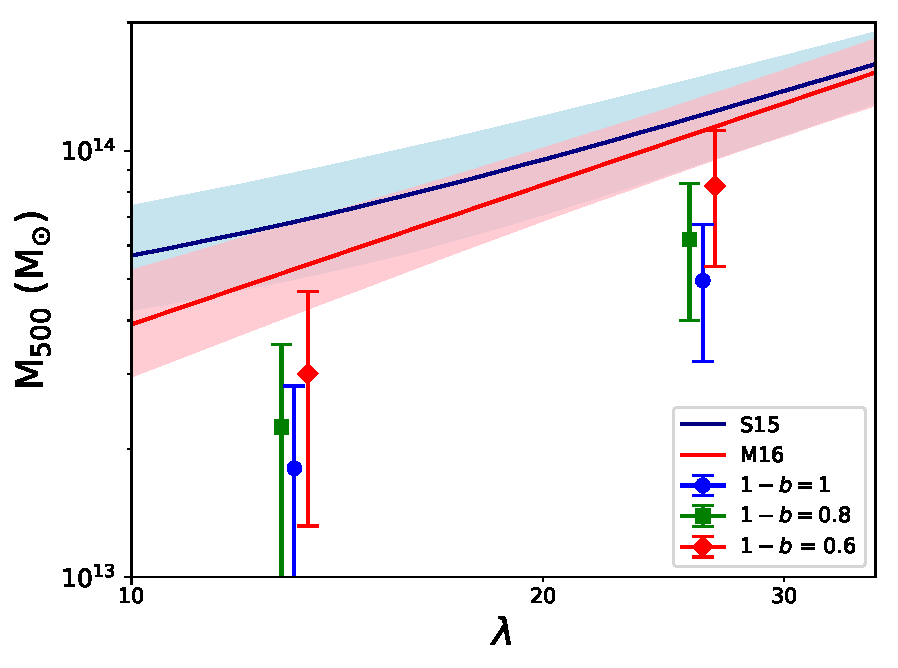
\includegraphics[width=\columnwidth] {M500_lambda_shela_sptvsrm.pdf}
  \caption{Comparison with redMaPPer mass-richness relations. The red line is the mass-richness relation of \protect \cite{2016arXiv161006890M} which was calibrated using weak-lensing masses of redMaPPer clusters in DES data. The blue line is the mass-richness relation of \protect \cite{2015MNRAS.454.2305S} which was calibrated using SZ masses of redMaPPer clusters in SPT. The data points for the results for the masses of the SHELA clusters in each richness bin with different values for the amount of hydrostatic mass bias, $1-b$. The data point for the case of $1-b=0$ is plotted at the average richness in each bin. The other two points are slightly offset from the average richness for the sake of clarity. For the two models, the redshift z = 0.7 is used.}
  \label{fig:y500vslambda}
\end{figure}


Accurately measuring the masses of cluster halos is necessary for clusters to be used for cosmology, making it is vital to map out the relation between mass and the cluster observables, such as the SZ signal and richness. It is important to compare different observable to mass relations which have different biases and contaminating factors to test if predicted scaling relations hold. Multiple studies have seen that the SZ observable has some feature that causes a lower SZ signal than predicted when $\lambda$--$M$ relations are extrapolated to lower mass objects \citep{2011A&A...536A..12P,2012PhRvD..85b3005D,2013ApJ...767...38S,2016arXiv160508770S}, and we explore that possibility here.  

\cite{2016arXiv160508770S} [S16] took a sample of DES redMaPPer clusters with weak lensing masses and measured their SZ signal in SPT (South Pole Telescope) data in multiple richness bins. They used weak lensing masses and their own richness-mass model \citep{2015MNRAS.454.2305S} [S15], which they inverted into a mass-richness model and extrapolated to measure $Y_{500}$. They ran two cases, using their own $M_{500} - Y_{500}$ model and using the model from A10. They compared the $Y_{500}$ expected in each richness bin to what was measured from stacking on the SPT SZ map. They found that for clusters with $\lambda$ > 80, $Y_{500}$ is consistent with their model and smaller by 0.61$\pm$0.12 from A10. For 20<$\lambda$<80, they found that the SZ signal was smaller by a factor of ~0.2-0.8, with higher richness bins and the S15 $M_{500} - Y_{500}$ showing better agreement. They explained this with a richness dependent bias, caused by contamination of the SZ and richness observables or bias in estimated halo mass, e.g. contamination of richness from line of sight projections, contamination of the SZ observable, a larger offset in SZ-optical centering than accounted for, or a larger intrinsic scatter in richness-mass relation at lower richness.
In Figure \ref{fig:y500vslambda} we compare our results to the $Y_{500}$-$\lambda$ relation of S16. To make this comparison, we need to take into account that they have modeled $P(\lambda|M_{500})$ as opposed to $P(M_{500}|\lambda)$. Their model is a log-normal distribution with mean:
\begin{equation}
\langle \ln\lambda | M_{500},z\rangle = \ln A_{\lambda} + B_{\lambda} \ln\bigg(\frac{M_{500}}{3 \times 10^{14}h^{-1}\rm M_{\odot}}\bigg) + C_{\lambda}\ln\bigg(\frac{E(z)}{E(z=0.6)}\bigg)
\end{equation}
To invert this relation, we perform the following operation:
\begin{equation}
P(M_{500}|\lambda^{\rm obs}) \propto P(M_{500},z) \int P(\lambda^{\rm obs}|\lambda) \  P(\lambda|M_{500},z) \ d\lambda
\end{equation}
where $P(\lambda|M_{500},z)$ is the SPT probability marginalized over the fit parameters $A_{\lambda}$, $B_{\lambda}$, and $C_{\lambda}$. $P(\lambda^{\rm obs}|\lambda)$ is the probability for observing a value for the richness given the true richness, and $P(M_{500},z)$ is proportional to the halo mass function. 


\cite{2016arXiv161006890M} [M16] measure the $P(M_{200}|\lambda)$ for redMaPPer clusters in DES. For comparison, we translate their model in terms of $M_{200m}$ to $M_{500c}$, where $m$ denotes the density contrast relative to the mean matter density and $c$ is relative to the critical density at that redshift. Although we do not compare our data to other redMaPPer richness-mass models, we note that there is good agreement with relations from S16 and \cite{2017MNRAS.466.3103S} [S17], which calibrates the mass-richness relation for redMaPPer clusters in SDSS.

We compare the models from S16 as they used redMaPPer clusters with masses derived using the SZ effect, as are ours, and M16 as their redMaPPer richnesses are from data observed by DECam, similarly to the SHELA data. Our data are plotted against these models in Figure \ref{fig:y500vslambda}. For the SHELA sample, $M_{500}$ from SZ profile fitting and the average richness per bin are used. We tested different ways to represent our richness bins, such as using mass-weighted and SZ-weighted average richnesses, but find that they are similar to the mean richness per bin, so we simply use the mean value. The average richnesses for the lower and higher richness bins are $\sim$13 and $\sim$26. Similarly to the results of S16, we find that our clusters are less massive than predicted. Relative to the model of S16: Our masses are 3.8 times smaller for the lower richness bin, and 2.5 times smaller for the higher richness bin, without accounting for hydrostatic mass bias. Relative to M16: Our masses are 2.9 times smaller for the lower richness bin, and 2.2 times smaller for the higher richness bin. If accounting for a hydrostatic mass bias of 0.8, our masses are 3.0 and 2.0 times smaller than S16 and 2.3 and 1.8 times smaller than M16, respectively for the lower and richness bin.
As is shown in Figure \ref{fig:y500vslambda}, a large value for hydrostatic mass bias is necessary to reconcile our data with the richness-based mass models. It would not be possible for an error in the richness to cause this large of a discrepancy, therefore there must be other factors in play. Several reasons are more contamination in the SZ signal than we have accounted for, mass-richness relations being incorrect at low richness, and differences in the meaning of the richnesses themselves because the objects are higher redshift and include IR data in the cluster finding algorithm.

%%%%%%%%%%%%%%%%%%%%%%%%%%%%%%%%%

%%%%%%%%%%%%%%%%%%%%%%%%%%%%%%%
%CONCLUSIONS
%%%%%%%%%%%%%%%%%%%%%%%%%%%%%%%
\section{Discussion} \label{sec:conclusions}
We have presented the analysis of stacked SZ profiles for a sample of IR and optically-selected clusters from the Spitzer-HETDEX Exploratory Large Area survey. We binned this sample into two richness bins: $10 \leq \lambda < 20$ and $\lambda \geq 20$. There are 623 clusters in the lower richness bin, and 75 in the higher richness bin. 
At the SZ null (220 GHz), the stacked profiles both exhibited an excess signal, which we attributed to thermal dust emission from cluster member galaxies. We tested for radio emission as well, but found no significant contribution.  For each bin, we fit for a dust SED using sources from the Herschel Stripe 82 survey catalog to extrapolate the dust SED from 220 GHz to 148 GHz, so that we could use the 220 GHz stacked profile as a template to clean the 148 GHz stack. As a check, we compared the ratio of dust emission at 148 and 220 GHz from the dust SED to the extrapolation from the Planck CIB power spectrum. We found a similar result for both methods, which is that $\sim28\%$ of thermal dust emission at 220 GHz is also present at 148 GHz. 
After removing dust emission, we fit the cleaned stack at 148 GHz to an SZ profile using a universal galaxy cluster pressure profile to translate our temperature decrement to a halo mass. For each richness bin, we used a MCMC procedure that simultaneously fit for the SZ profile and dust SED while fixing redshift to the average of the cluster sample.  We compared the chains with and without the dust correction, and found for the lower richness bin, $10 \leq \lambda < 20$, that correcting for dust emission increases the $M_{500}$ measurement by a factor of 1.9. For the higher richness bin, $\lambda 
\geq 20$, $M_{500}$ increases by a factor of 2.2. This translates to 80\% $\pm$ 65\% of the SZ signal in the lower richness bin and 65\% $\pm$ 40\% of the SZ signal in the higher richness bin being filled in by dust emission. 

\iffalse
The SHELA cluster catalog contains stellar masses from FAST and richnesses from redMaPPer. We used this information, along with our SZ masses, to compare the SHELA clusters to other works in the literature. 
We measured $f^*_{500}$, the fraction of stellar mass to total mass within a radius of $R_{500}$, using cluster member galaxies' stellar masses and probabilities of cluster membership. We found a stellar mass fraction that decreases with increasing halo mass, agreeing with what has been found with previous studies. We found that $f^*_{500}$ is lower than in previous studies, $2.9\%$ and $1.9\%$ \textbf{+errors} for the lower and higher richness bins, respectively. 
\fi
The SHELA cluster catalog obtains richnesses from the redMaPPer algorithm. We used this information, along with our SZ masses, to compare the SHELA clusters to other works in the literature. 
We compared our mass and richness data to two models which have mapped out the richness-mass relation for redMaPPer clusters. SZ measurements of optically-selected clusters are generally smaller than expected when comparing to mass-richness models, and the SHELA clusters follow this trend. We found that our data are 3.8 and 2.5 times smaller than predicted, respectively for the lower and higher richness bins relative to the model of S15. In comparison to the model of M16, our masses are 2.9 and 2.2 times smaller for the lower and higher richness bins, respectively.

This is a step toward studying characteristics of galaxy clusters over a range of redshifts and masses. In the future, wider and deeper coverage by Advanced ACT and the Simons Observatory will allow this study by observing a large number of clusters in five frequency bands, and by increasing overlap with optical surveys such as BOSS, HSC, DES, DESI, and LSST \citep{2016SPIE.9910E..14D}. In the future it may be fruitful to repeat this type of analysis for more infrared-selected objects, using the Spitzer IRAC Equatorial Survey \citep[SpIES,][]{2016ApJS..225....1T}. SpIES is shallower than SHELA, but larger, covering an adjacent $\sim$115 square degrees of Stripe 82.

\section*{Acknowledgments}
BJF and KMH acknowledge support by the National Aeronautics \& Space Administration through the University of Central Florida's NASA Florida Space Grant Consortium and Space Florida.  This work was supported by the U.S. National Science Foundation through awards AST-0408698 and AST-0965625 for the ACT project, as well as awards PHY-0855887 and PHY-1214379. Funding was also provided by Princeton University, the University of Pennsylvania, and a Canada Foundation for Innovation (CFI) award to UBC. ACT operates in the Parque Astron\'omico Atacama in northern Chile under the auspices of the Comisi\'on Nacional de Investigaci\'on Cient\'ifica y Tecnol\'ogica de Chile (CONICYT). Computations were performed on the GPC supercomputer at the SciNet HPC Consortium. SciNet is funded by the CFI under the auspices of Compute Canada, the Government of Ontario, the Ontario Research Fund - Research Excellence; and the University of Toronto. The development of multichroic detectors and lenses was supported by NASA grants NNX13AE56G and NNX14AB58G. We thank our many colleagues from ABS, ALMA, APEX, and Polarbear who have helped us at critical junctures. Colleagues at AstroNorte and RadioSky provide logistical support and keep operations in Chile running smoothly. We also thank the Mishrahi Fund and the Wilkinson Fund for their generous support of the project. %MCMC parameter contours were plotted using the python package \textit{corner} \citep{corner}.
\textbf{SHELA Acknowledgments}

%%%%%%%%%%%%%%%%%%%%%%%%%%%%%%%%%%%%%%%%%%%%%%%%%%

%%%%%%%%%%%%%%%%%%%% REFERENCES %%%%%%%%%%%%%%%%%%

% The best way to enter references is to use BibTeX:

\bibliographystyle{mnras}
\bibliography{shela_sz} 


%%%%%%%%%%%%%%%%%%%%%%%%%%%%%%%%%%%%%%%%%%%%%%%%%%


% Don't change these lines
\bsp	% typesetting comment
\label{lastpage}
\end{document}
